\documentclass[10pt]{article}
\pdfoutput=1 

\addtolength{\oddsidemargin}{-.875in}
\addtolength{\evensidemargin}{-.875in}
\addtolength{\textwidth}{1.75in}

\addtolength{\topmargin}{-.875in}
\addtolength{\textheight}{1.75in}

\openup 1em

%macro for commenting
\usepackage{color}
\newcommand{\leo}[1]{{\color{blue}{\it leo: #1}}}

\newcommand{\Xbeta}{ X_i^T \beta}
\newcommand{\xbeta}{ x_i^T \beta}
\newcommand{\xbetaij}{ x_{ij}^T \beta}
\newcommand{\sgamma}{s_{ij}^T\gamma_i}

\usepackage[round]{natbib}

\usepackage{rotating}
\usepackage{graphicx}
\usepackage{subcaption}

\usepackage{float}


\usepackage{amsthm,amsmath} 
\usepackage{amssymb}
\usepackage{subcaption}

\newtheorem{theorem}{Theorem}
\newtheorem{lemma}{Lemma}
\newtheorem{corollary}{Corollary}
\newtheorem{remark}{Remark}


\usepackage{algorithm}
\usepackage{algpseudocode}


\thispagestyle{empty}
\baselineskip=28pt

\title
{{Calibrated Data Augmentation for Scalable \\ Markov Chain Monte Carlo}}


\author{
     Leo L. Duan,
     James E. Johndrow,
     David B. Dunson
    % \textsuperscript{*}\footnotemark[2]\and
}

 
\begin{document}
    
\maketitle

{\bf Abstract:} Data augmentation (DA) is a common technique for building tuning-free Markov chain Monte Carlo algorithms. Although these algorithms are very popular, 
autocorrelations are often high in large samples, leading to poor computational efficiency.  This phenomenon has been attributed to a mismatch between the rate of convergence of the posterior distribution conditionally on augmented data and with augmented data marginalized out.  In this article, we propose a calibrated DA (CDA) algorithm, which adjusts for this mismatch by slowing down the convergence of the conditional distribution via parameter marginalization or scale increasing. The bias introduced by changing the scale can be eliminated through a Metropolis-Hastings step, or in some cases, analytically bounded with suitable working parameters. CDA is easily applied to a broad variety of existing DA algorithms, and we focus on three popular models: probit, logistic and Poisson log-linear.  Theoretical support is provided and dramatic gains are shown in applications.
\vskip 12pt

%\baselineskip=12pt
%\par\vfill\noindent
{\noindent  KEY WORDS:  Albert and Chib; Approximate Markov chain Monte Carlo; Big $n$; Data Augmentation; Maximal Correlation; Polya-Gamma; Scaling limits.}
%\par\medskip\noindent
%\clearpage\pagebreak\newpage
\pagenumbering{arabic}

\section{Introduction}

With the deluge of data in many modern application areas, there is a pressing need for scalable computational algorithms for inference from such data, including uncertainty quantification (UQ).  Somewhat surprisingly, even as the volume of data increases, uncertainty often remains sizable.  Examples include financial fraud detection \citep{ngai2011application}, disease mapping \citep{wakefield2007disease} and online click-through tracking \citep{wang2010click}.  Bayesian approaches provide a useful paradigm for quantifying uncertainty in inferences and predictions in broad settings.

The standard workhouse for Bayesian posterior computation is Markov chain Monte Carlo (MCMC), and related sampling algorithms. Non-sampling alternatives, such as variational Bayes, tend to lack accuracy guarantees. However, it is well known that conventional MCMC algorithms are often unscalable for computation with large and complex data. Due to the iterative nature, the computational cost is the product of two factors: the evaluation cost at each sampling iteration and the total number of iterations needed to obtain an acceptably low Monte Carlo error.  As an analogy to travel in the real world, the former is the speed and the latter is the path distance to reach and tour the target.  Any scaling obstacle in either factor will make MCMC inapplicable. 

In recent years, a rich literature has developed focusing on increasing speed (\cite{minsker2014robust,srivastava2015wasp,conrad2015accelerating} among others), mainly through accelerating or parallelizing the sampling procedures at each iteration.  However, very little attention has been paid to the problem of finding an efficient path to reach and explore the target distribution in big data settings. This issue is of substantial practical performance, as many routinely used algorithms, such as data augmentation samplers for probit \citep{albert1993bayesian} and logistic models \citep{polson2013bayesian}, can suffer from extreme slow mixing for large sample sizes and become unusable as sample size increases (see \cite{rajaratnam2015mcmc} and \cite{johndrow2016inefficiency} for details).

Such issues provide motivation for the development of algorithms for accelerating mixing in large sample size $n$ settings.  In this article, we focus on improving data augmentation (DA) based MCMC algorithms.  Letting $\pi( \theta | y )$ denote the posterior distribution of the parameters $\theta$ given data $y$, such algorithms focus on the modified stationary distribution $\pi( \theta, z | y ),$ with latent data $z$ introduced in a careful manner so that $\pi( \theta | y) = \int \pi( \theta, z | y ) dz$ and posterior sampling based on the conditional posterior distributions $\pi(z | \theta, y)$ and $\pi( \theta | z, y)$ is easier than directly sampling based on $\pi( \theta | y)$.   For example, after data augmentation a simple blocked Gibbs sampler may be possible, while sampling based on the non-augmented posterior $\pi( \theta |y)$ may require substantial tuning.  DA algorithms are used routinely, with the algorithms of \cite{albert1993bayesian} for probit models and \cite{polson2013bayesian} for logistic regression and Poisson log linear models particularly popular.  

The broad use of such DA algorithms is well justified given their simplicity, lack of tuning and good performance in a broad variety of settings.  However, as the sample size $n$ increases, substantial mixing problems can arise due to a mis-calibration issue.  In particular, it is often the case that as $n$ increases, the conditional posterior $\pi( \theta | z, y)$ concentrates at a faster rate than the marginal posterior $\pi( \theta | y)$. {\color{red} With $\pi(  z|\theta y)$ strongly dependent on the previous state of $\theta$}, this can cause the step size of MCMC algorithms for updating $\theta$  to be much too small.  Special cases of this pitfall of DA are well known in the literature.  For example, the \cite{albert1993bayesian} DA algorithm for probit models for ordered categorical data updates latent threshold parameters from their uniform conditional posterior given the augmented data.   As $n$ increases, these uniform distributions have small support heavily correlated with the previous threshold value, leading to critical mixing problems even in moderate samples.  In this specialized setting, it is common to marginalize out $z$ in updating the latent thresholds using a Metropolis-Hastings (MH) step \citep{cowles1996accelerating}. In this article, our focus is on obtaining a broad and more fundamental solution to the mis-calibration problem.

There is a previous literature attempting to accelerate mixing in DA algorithms through the use of parameter expansion (PX) \citep{liu1999parameter}.  The basic idea of PX-DA is that poor mixing is often due to high posterior dependence in parameters, which are updated separately within an MCMC algorithm.  By introducing extra or redundant parameters into the MCMC algorithm, it is possible to dilute correlations in the parameters of interest and obtain improved mixing.  PX-DA versions of the popular \cite{albert1993bayesian} algorithm have been developed \citep{liu1999parameter}, leading to some gains.  

However, PX-DA does not address the mis-calibration issue, which is the focus of this article.  In particular, we propose a calibrated DA (CDA) class of algorithms, which {\color{red} removes the dependency of the latent variable on the parameter, or} calibrates the transition variance in the posterior $\pi( \theta | z, y)$ by adjusting the conditional variance.  These adjustments can very significantly reduce autocorrelation in the Markov chain, dramatically improving mixing relative to DA or PX-DA in many very large $n$ settings. Calibrating the variance leads to a bias in the stationary distribution so that the target is $\pi_r( \theta | y)$, which may differ slightly from $\pi( \theta | y)$.  Metropolis-Hastings adjustment is employed to eliminate bias. We also show in several cases, this approximation error can be analytically bounded with suitable choice of the working parameter, leading to fast-mixing approximate MCMC. The proposed CDA approach is widely applicable, and we demonstrate the utility through probit, logistic and Poisson log-linear examples.


Section 2 proposes the general calibrated data augmentation (CDA) algorithm. Section 3 presents theory showing acceleration of mixing, accuracy of approximation, and ergodicity for the approximate MCMC algorithm without use of a MH adjustment.  Section 4 provides simulation experiments and comparisons with existing algorithms.  Section 5 contains an application to a large computational advertising data set. All the proofs are provided in the appendix. %check again

\section{Calibrated Data Augmentation}

The primary role of data augmentation (DA) in MCMC algorithms is to make Gibbs sampling possible, because after augmentation conditional posterior distributions follow parametric forms that are easy to sample from.  DA Gibbs proceeds by sampling from the conditional posterior distributions of the latent data based on $\pi(z| \theta,y)$ and from conditional posterior distributions of the parameters based on $\pi(\theta | z,y)$; each of these sampling steps can be broken up into a series of conditional updates for successive subsets of the latent data and parameters when the joint conditionals $\pi(z|\theta,y)$ and $\pi(\theta | z, y)$ are not available in a simple form.

The current article focuses on problems that arise due to a mis-calibration problem that occurs when {(i) \color{red} $z$ is strongly dependent on the last value of $\theta$, and (ii) $\mbox{var}(\theta | z,y)$ is substantially less than $\mbox{var}( \theta | y)$.  The first condition is very common in Gibbs sampling due to the use of full conditional distributions.} The second condition is related to the rate difference of the concentration.  Consider that the conditional posterior given the latent data is obtained by updating the posterior given the observed data with information in the latent data likelihood via Bayes rule as: $\pi( \theta | z, y) \propto \pi( \theta | y) L( z | \theta, y)$.  Hence, as the amount of information in the latent data likelihood $L(z | \theta, y)$ increases, which typically occurs as the observed data sample size $n$ increases, $\mbox{var}(\theta | z,y) \ll \mbox{var}( \theta | y)$.  The combination of these two conditions naturally leads to a slow mixing problem, because the MCMC updates based on $\pi(\theta | z,y)$ will only explore a small region of $\pi( \theta | y)$.  In general, the problem gets worse as the information in the latent data likelihood increases; inefficiency can arise even in moderate sample sizes but becomes critical in large samples.

The key novel idea of this article is to {\em calibrate} DA by adjusting the step size of the conditional distribution. Addressing either one of the conditions mentioned above leads to substantial acceleration. To remove the dependency of the latent variable on the last state,  the calibrated DA (CDA) first marginalizes out the parameter from the Markov chain and then samples the parameter as an extra step at the end of each iteration. To calibrate the rate mismatch in the conditional posterior covariance, CDA induces an increase in $var( \theta | z,y)$ by  inflating the variance parameter with a working parameter $r$. This leads up to an altered likelihood $\pi_r(y|\theta)= \int \pi_r(y|\theta,z)\pi_r(z)dz$. To reduce the bias, a correction term $b$ is introduced so that $\pi_{r,b}(y|\theta)$ is close to $\pi(y|\theta)$. The samples from $\pi_{r,b}(y|\theta)$ can be used as either as approximate posterior or good proposal in the Metropolis-Hastings algorithm. We demonstrate a general numeric algorithm for $\pi(\theta | y,z)$ in the location-scale family, as well as analytical method for some special cases.

We now illustrate the two calibration strategies. As the parameters are commonly in multiple dimensions, we now divide the parameter into two sets $\theta=\{\theta_1,\theta_2 \}$. Let $\theta_1$ be the ones that mixes slowly.



\subsection{Removing Dependency by Marginalization}

Intuitively, if $\theta_1$ concentrates rapidly near a function of $z$, but $z$ depends on the last value of $\theta_1$, slow mixing naturally occurs. Breaking the dependency would lead to significant improvement. The first strategy involves marginalize out $\theta_1$ in the conditional distribution of  $z$ and $\theta_2$, then  sample new $\theta_1$ based on $\pi(\theta_1|z,\theta_2,y)$, shown in Algorithm~\ref{integration_cda}:

\begin{algorithm}[H]
		\caption{Marginalization based CDA}
		\label{integration_cda}
		    \begin{algorithmic}
		\State Based on the augmented joint distribution $\pi (z,y,\theta_1,\theta_2)$, obtain the marginal $\pi (z,y,\theta_2)=\int\pi (z,y,\theta_1,\theta_2) d\theta_1$.
		\State \For{ $step=1\ldots N_{Steps}$ }
		\State Sample $z$ from the marginal $\pi(z|\theta_2, y)$;
		\State Sample $\theta_2$ from the marginal $\pi(\theta_2|z, y)$;
		\State Sample $\theta_1$ from the full conditional $\pi(\theta_1|z,\theta_2, y)$;
		\EndFor
		\end{algorithmic}
\end{algorithm}

Obviously, this does not change the stationary distribution, but the sampling of the latent variable $z$ no longer relies on the previous value of $\theta_1$. Therefore the generation of the new $\theta_1$ is free from its last state.

This integration strategy is similar to the collapsed sampler proposed by \cite{liu1994collapsed},  who focused on accelerating the imputation of $z$ as the missing data by marginalizing out the the unimportant variables. The key difference is that $\theta_1$ is important but marginalized out at first to exclude the information of the past, then it is sampled again at the end of each MCMC iteration. Note the first two steps in the algorithm  already form a complete Markov chain and neither $\pi(z|\theta_2, y)$ or $\pi(\theta_2|z, y)$ depends $\theta_1$. Therefore the autocorrelation of $E(\theta_1|z,\theta)$ is significantly reduced. A more rigorous theory will be provided in the next section.

\begin{remark}
	Due to the closed-form of $\pi(\theta_1| \theta_2,z,y)$ is commonly available in Gibbs sampling, it is possible to marginalize $\theta_1$ out in most cases. The easiness of applying the new algorithm depends on if the marginal $\pi(z|\theta_2, y)$ and $\pi(\theta_2|z, y)$ can be readily sampled. When this is not true, it is possible to make some compromises such as reverting $\theta_2$ to $\pi(\theta_2|\theta_1,z, y)$, as long as $\theta_2$ does not impact greatly on the concentration of $\theta_1$.
	\end{remark}

We use the next example to show if $\pi(\theta_1| \theta_2,z,y)$  follows uniform distribution, the marginalization does not alter the distribution forms of the other posteriors, but leads to significant gains in mixing. Therefore, under such cases marginalization is always recommended.

{\bf Example 1: Threshold Updating in Ordinal Probit Regression}

Consider the \cite{albert1993bayesian} DA algorithm for the probit regression with ordered categorical data, as aforementioned in the introduction. The likelihood is $L(y_i=j|x_i,\beta,\gamma)= \{  \Phi( \gamma_j- x^T_i\beta) -  \Phi( \gamma_{j-1}- x^T_i\beta)    \}$, where $\Phi$ is the cumulative distribution function of standard normal, $\gamma=\{\gamma_0,\gamma_1,...\gamma_k\}$ are the threshold parameters that correspond to the boundaries of $k$ categories, with $\gamma_0=-\infty$, $\gamma_k=-\infty$. To ensure identifiability, $\gamma_1$ is fixed at $0$. A latent variable was discovered as the truncated normal distribution conditioned on $\beta$ and $\gamma$, $z_i \sim \mathcal N_{(\gamma_{j-1}, \gamma_{j})}(x^T_i\beta,1)$. For simplicity, flat priors are assumed for both $\beta$ and $\gamma$. Thanks to the augmentation, the posterior for the other parameters  can be sampled from  normal $\beta \sim \mathcal{N} \{   (x^Tx)^{-1}(x^Tz),(x^Tx)^{-1} \}$ and uniform $\gamma_j \sim \mathcal{U}\{ \underset{i:y_i=j}{\max}(z_i),  \underset{i:y_i=j+1}{\min} (z_i)  \}$.

In the conditional distribution $\pi( z|\gamma,\beta,y) $, both the maximum of $z_i \sim \mathcal N_{(\gamma_{j-1}, \gamma_{j})}(x^T_i\beta,1)$ and the minimum of $z_i \sim \mathcal \mathcal{N}_{(\gamma_{j}, \gamma_{j+1})}(x^T_i\beta,1)$ approach rapidly to the boundary $\gamma_j$ as the numbers of $y_i=j$ and $y_i=j+1$ increase. Immediately at the next step,  $\pi( \gamma_j| z,y) $ is confined by those two values. This causes critical mixing issue. To illustrate, we simulate only $1,000$ data points with $x_i^T\beta \sim \mathcal{N}(-1,1)$ and threshold $\{-\infty, 0, 1, \infty\}$, obtaining 3 categories with count $504$, $267$ and $229$. Even on this small sample with relatively balanced data, the estimated threshold $\gamma_2$ is critically slow (Figure~\ref{ordered_probit}).

Following Algorithm~\ref{integration_cda} with $\theta_1=\{ \gamma_2,\ldots \gamma_{k-1}\}$ and $\theta_2=\beta$, CDA first integrates the joint distribution $\pi(z,y,x,\beta,\gamma,y)= \prod_i  {\mathcal N} (z_i |x^T_i\beta,1)   \prod_{j=1} \frac{1 \{ \underset{i:y_i=j}{\max}(z_i) < \gamma_j< \underset{i:y_i=j+1}{\min} (z_i) \}}{\underset{i:y_i=j+1}{\min} (z_i) -\underset{i:y_i=j}{\max}(z_i) }$ over $\gamma_2,\ldots \gamma_{k-1}$, where each uniform simply integrates to $1$. The resulting algorithm is 

\begin{equation}
	\begin{aligned}
	&	z_i \sim  {\mathcal N}_{(-\infty,0)} (x^T_i\beta,1) \text{ if $y_i=1$},\\
	&	z_i \sim {\mathcal N}_{(0,\infty)} (x^T_i\beta,1) \text{ if $y_i>1$},\\
	&	\beta \sim \mathcal{N} \{   (x^Tx)^{-1}(x^Tz),(x^Tx)^{-1}  \} ,\\
	& \gamma_j\sim U(  z_{\big(\sum_i 1(y_i \le j) \big)}, z_{\big(\sum_i 1(y_i \le j)+1 \big)}), 
	\end{aligned}
\end{equation}
where $z_{\big(m\big)}$ denotes the $m$th order statistics. Due to the removal of correlation from the past, the mixing is substantially improved (Figure~\ref{ordered_probit}).



\begin{figure}[H]
 % \centering
  \begin{subfigure}[b]{0.49\textwidth}
 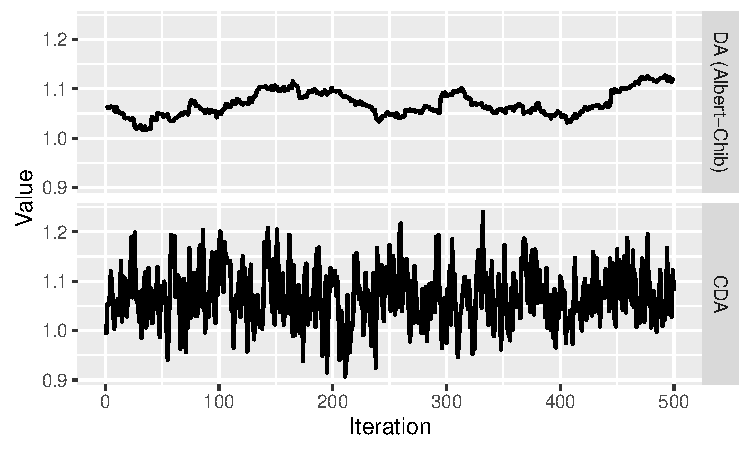
\includegraphics[width=1\textwidth]{ordered_probit_trace_plot.pdf}
  \caption{Traceplot illustrating mixing performance of the original DA and CDA algorithms in the threshold updating in probit regression with ordered categorical data.}
\end{subfigure}
  \hfill
   \begin{subfigure}[b]{0.49\textwidth}
 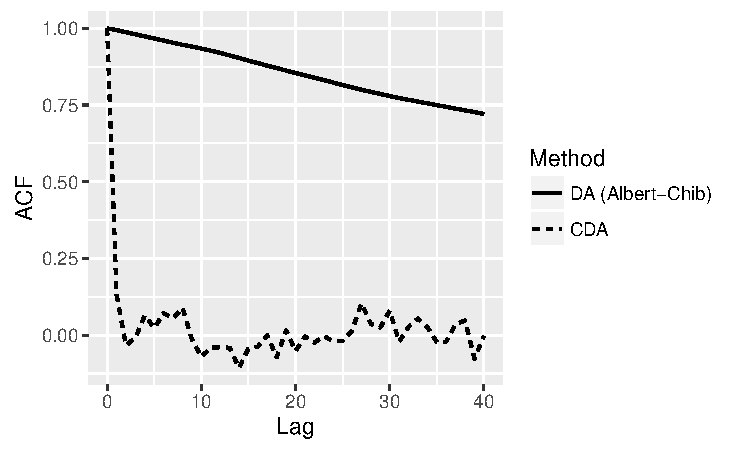
\includegraphics[width=1\textwidth]{ordered_probit_acf.pdf}
  \caption{Autocorrelation function (ACF) illustrating that the calibration improves the mixing from high correlation in $40$ lags to an immediate drop to low correlation.  
  }¡
\end{subfigure}
 \caption{Panel (a) demonstrates the improvement in mixing and panel (b) shows autocorrelations change by calibrating  \cite{albert1993bayesian} algorithm with threshold updating in ordered categorical data.}
  \label{ordered_probit}
 \end{figure}
 

\subsection{Fixing Variance Mismatch by Increasing Conditional Variance}

CDA can directly correct the mismatch between the marginal and conditional variances. This relies on increasing the conditional variance via an approximate distribution. We assume the adjusting does not impact the posterior of $\pi(\theta_2|\theta_1,z,y)$, for notational simplicity, we use $\theta$ to represent of $\theta_1$ and omit $\theta_2$ in this section. CDA first induces an increase in $var(\theta|z,y)$ by modifying the parameters in each $\pi(z_i|\theta)$ with an working parameter $r_i$. For example,  when $var(\theta|z,y)$ is a linear function of the $var(z_i|\theta)$ (e.g. $var(\theta|z,y)= [ x^{T} diag \{ 1/ var(z_i|\theta)\}x ]^{-1}$), it is replaced with the $r_i  var(z_i|\theta)$; when $var(\theta|z,y)$ is related to $z_i$  (e.g.  $var(\theta|z,y)= [ x^{T} diag \{z\}x ]^{-1}$), we change the parameters in $\pi(z_i|\theta)$ to generate smaller $z_i$. Let subscript $r$ denote the modified ones. The modified marginal likelihood is obtained for each $L_r(y_i|\theta)= \int \pi(y_i, z_i | \theta) d z_i$. Without loss of generality, we assume that variance is monotonically increase in $r>1$ and $r=1$ corresponds to no change. 

With the same distributional form, the integration will have the same distribution as $L(y_i|\theta)$ with difference parameters. Comparing the two, a bias correction term $b_i$ is used to quantify the difference. For example, if $L(y_i|\theta)$ and $L_r(y_i|\theta)$ differs in the parameter as $x_i^T\theta$ and  $\sqrt{r_i} x_i^T\theta$, then the second term is replaced as $\sqrt{r_i} x_i^T\theta+ b_i$ with  ideal bias correction  near $(1-\sqrt{r_i}) x_i^T\theta$. Then new the correction parameter is passed down in deriving the posterior $\pi_{r,b}( z_i | y_i, \theta )$ and $\pi_{r,b}( \theta |z,y)$.  Note that although the exact bias $f_b(\theta,y_i, r_i)$ can be obtained as a function of $\theta$, one would not use it to correct bias at every step as it would cause convergence issue.

With fixed $r$ and $b$, the posterior sample from the new $\pi_{r,b}(\theta|y)$ is an approximate to the $\pi(\theta|y)$. To reduce the approximation error, the numeric adaptation can be made on $r_i$ and $b_i$ to increase $L_{r,b}(y_i\theta)/L(y_i|\theta)$. To obtain exact posterior, the sample from $\pi_{r,b}(\theta|y)$ can be used as proposal in Metropolis-Hastings step. Due to the similarity of the proposal to the true density, the proposed new parameter can be in multiple dimensions while enjoys high acceptance rate. In some special cases, analytical solution exists for good values of $r_i$ and $b_i$ with negligible approximation error, then the sample of $\pi_{r,b}(\theta|y)$ can be as the approximate posterior sample without the accept-reject step.

\subsubsection{Numeric Exact Method}

We first present a general method that works in most of the DA algorithms that requires calibration. This involves numeric adaptation of the working parameters $r$ and $b$. The algorithm is listed in Algorithm~\ref{numerical_cda}. After the variance and bias adjustment terms are included, the procedures consists of two parts: in the tuning period, $r$ and $b$ are adapted using $L_{r,b}(y_i\theta)/L(y_i|\theta)$ at each step; in the sampling period, those parameters are fixed to ensure ergodicity.
 
 
\begin{algorithm}[H]
		\caption{Variance Adjusting CDA (Numeric)}
		\label{numerical_cda}
		    \begin{algorithmic}
		\State Increase the variance of $\pi(\theta| z,y)$ by changing the parameter in $\pi(z_i |\theta,y_i)$ with $r_i$;
		\State Integrate the modified density to obtain $L_r(y_i|\theta)= \int \pi_r (z_i|\theta) \pi(y_i|z_i,\theta) d z_i$; 
		\State Compare with $L(y_i|\theta)$, include another bias correction parameter $b$ so that $L_{r,b}(y_i|\theta)$ can be equal to $L(y_i|\theta)$ with some $b$ for all $r$.
		\State Derive the analytical form of $f_b(\theta,y_i,r_i)$ so that $L_{r,b={f_b(\theta,y_i,r_i)}}(y_i|\theta)=L(y_i|\theta)$;
		\State Obtain $\pi_{r,b}(z_i|\theta, y_i)$ and  $\pi_{r,b}(\theta| z, y)$;
		\State Initialize $r_i$ to a large value and $b_i= f_b(\theta,y_i, r_i)$  for $i=1\ldots n$;
		\State \For{ $step=1\ldots N_{Steps}$ }
		\State Generate individual $z_i$ from $\pi_{r,b}(z_i|\theta, y_i)$;
		\State Generate $\theta'$ from $\pi_{r,b}(\theta'|z, y)$;
		\State Compute $\alpha_i = \frac{L( y_i|\theta', z_i ) }{L( y_i|\theta, z_i )}$  for $i=1\ldots n$;
		\State Set $\theta=\theta'$ if $\mathcal{U}(0,1)< \frac{Q(\theta',\theta)}{Q(\theta,\theta')}\prod \alpha_i$, where $Q(\theta,\theta') = \int  \pi_{r,b}(\theta| z, y) \pi_{r,b}(z|\theta', y)d z$
		\State \If{$step<N_{Tuning}$}
			\State Set $b_i= f_b(\theta,y_i, r_i)$ for $i=1\ldots n$;
			\State If $\alpha_i<1$, set $r_i$ to $1 \vee (r_i \alpha_i)$  for $i=1\ldots n$;
		\EndIf
		\EndFor
		\end{algorithmic}
\end{algorithm}

\begin{remark}
The algorithm is generally applicable. For example, in the cases where $\pi(z_i | \theta,y_i)$ is in location-scale family, the variance adjustment can be made on the scale parameter while bias correction is applied on the location parameter. In most cases, $\frac{Q(\theta',\theta)}{Q(\theta,\theta')}=1$ due to the symmetry.
\end{remark}

We now use the probit regression to illustrate the numeric method. Due to the conditional $\pi(z_i | \theta,y_i)$ is normal, CDA increases its variance and applies bias correction on the mean.

 {\bf Example 2: Probit Regression with Rare Event}

 
Consider a probit regression $\prod_{i=1}^{n}L(y_i|\xbeta)= \prod_{i=1}^n \Phi(\xbeta)^{y_i} \{ 1-\Phi(\xbeta) \} ^{(1-y_i)}$ with rare event so that the total occurrence of $y_i=1$ is quite small compared to to $n$. We use $\beta={-5,1}$ corresponding to the intercept and $x_{i,1}\sim \mathcal{N}(0,1)$ to generate only $29$ positive outcomes among $n=10,000$. The posterior samples from $\beta \sim \mathcal{N} \{   (x^Tx)^{-1}(x^Tz),(x^Tx)^{-1} \}$, conditional on $z_i \sim N_{(-\infty,0)}(\xbeta,1)$ if $y_i=0$ and $z_i \sim N_{(0,\infty)}(\xbeta,1)$ if $y_i=1$. For the intercept term, it concentrates at the rate of $O(1/n)$; while marginally, it concentrates much slower at $O(1/\log n)$. The slow mixing becomes particularly problematic when $n$ is very large, which is common in rare event applications. In this testing case, the \cite{albert1993bayesian} DA algorithm suffers from extremely slow mixing. To compare, we test the parameter expansion algorithm (PX-DA) proposed by \cite{liu1999parameter}, where a redundant parameter is used in the probit link $\Phi(\alpha\xbeta)$. PX-DA reduces the correlation to some extent, however, it does not solve the variance mismatch problem. As shown in Figure~\ref{probit_demo} (a) and (b), both DA and PX-DA result in extremely slow mixing.

Noting $var(z_i| \beta)=1$, CDA algorithm first replaces the it with $r_i > 1$ so that the conditional variance for $\beta$ becomes $(x^T diag^{-1}\{r_i\} x)^{-1}$. The marginalization and adding bias correction leads to $L_{r,b}(y_i|\beta)= \Phi\{  (\xbeta+ b_i)/\sqrt{r_i}  \}^{y_i} [ 1-\Phi\{  (\xbeta+ b_i)/\sqrt{r_i}  \} ] ^{(1-y_i)}$. The resulting algorithm for the proposal is:
 
\begin{equation}\begin{aligned}
&	  z_i \sim N_{(-\infty,0)}(\xbeta+b_i,r_i) \text{ if $y_i=0$ } \\
&	  z_i \sim N_{(0,\infty)}(\xbeta+b_i,r_i) \text{ if $y_i=1$}\\
&    \beta \sim \mathcal{N} \{   (x^T diag^{-1}\{r_i\}x)^{-1},  x^T diag^{-1}\{r_i\}(z-b_i),(x^T  diag^{-1}\{r_i\} x)^{-1} \} 
\end{aligned}\end{equation}

 The calibrated algorithm leads to significant improvement of the mixing (Figure~\ref{probit_demo}a and b). In the numerically adapted proposal distribution (that is close to the true posterior distribution), it is interesting to note the tuned $r_i$ is related to the posterior value of $\xbeta$ (Figure~\ref{probit_demo}c). The very negative $\xbeta$ ($< -4$) suffers the mis-match in the conditional and marginal variance, hence allows large $r_i$ to adjust the step size. The bias correction is linear in $(\sqrt{r_i}-1 ) \xbeta$ as expected (Figure~\ref{probit_demo}d).
 
 
\begin{figure}[H]
 % \centering
  \begin{subfigure}[b]{0.49\textwidth}
 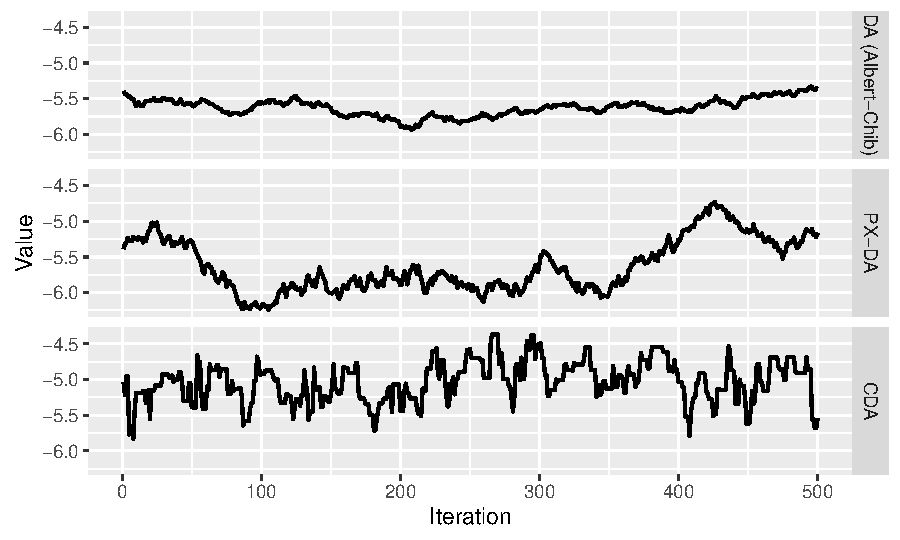
\includegraphics[width=1\textwidth]{probit15_trace_plot.pdf}
  \caption{Traceplot illustrating mixing performance of the original DA, parameter expanded DA and CDA algorithms in probit regression with rare event data.}
\end{subfigure}
  \hfill
   \begin{subfigure}[b]{0.49\textwidth}
 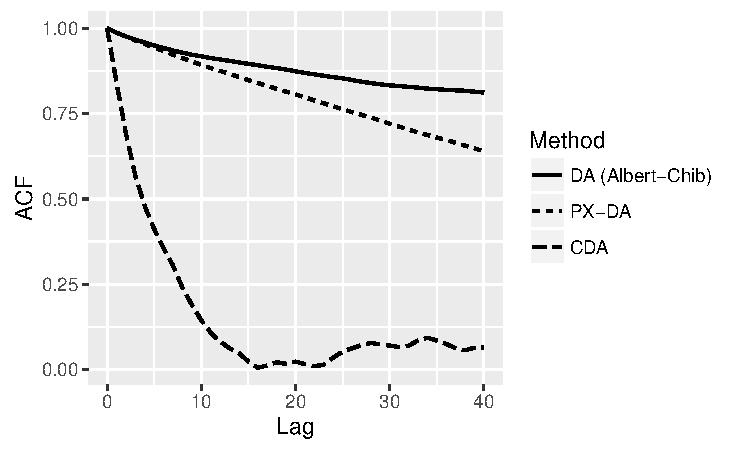
\includegraphics[width=1\textwidth]{probit15_acf.pdf}
  \caption{Autocorrelation function (ACF) illustrating the slow mixing of the DA and parameter expanded DA in rare event data, and CDA correcting this problem.}
\end{subfigure}
   \begin{subfigure}[b]{0.49\textwidth}
 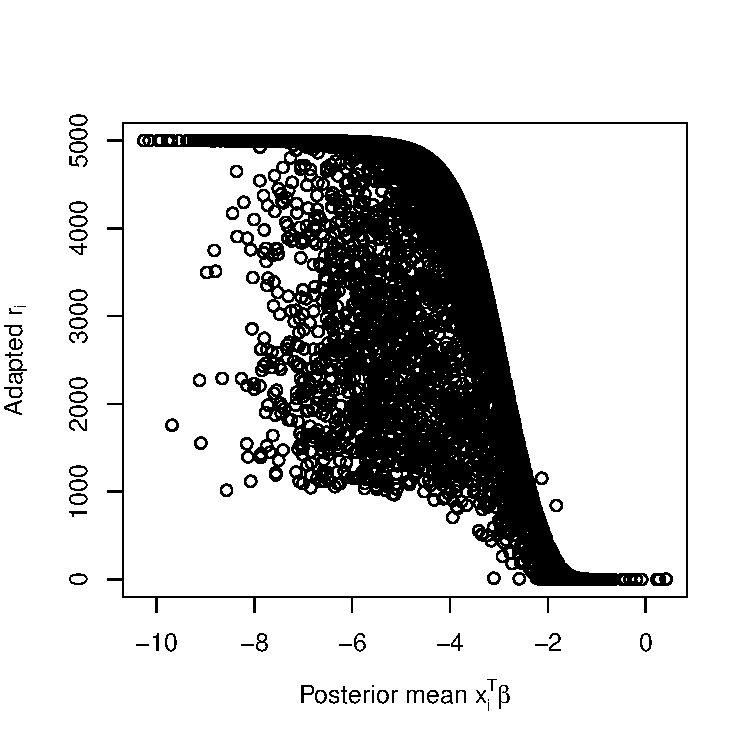
\includegraphics[width=1\textwidth]{probit_cda_r}
  \caption{Numerically optimized $r_i$ showing the room for variance increase is related to the  value of $\xbeta$.}
\end{subfigure}
  \begin{subfigure}[b]{0.49\textwidth}
 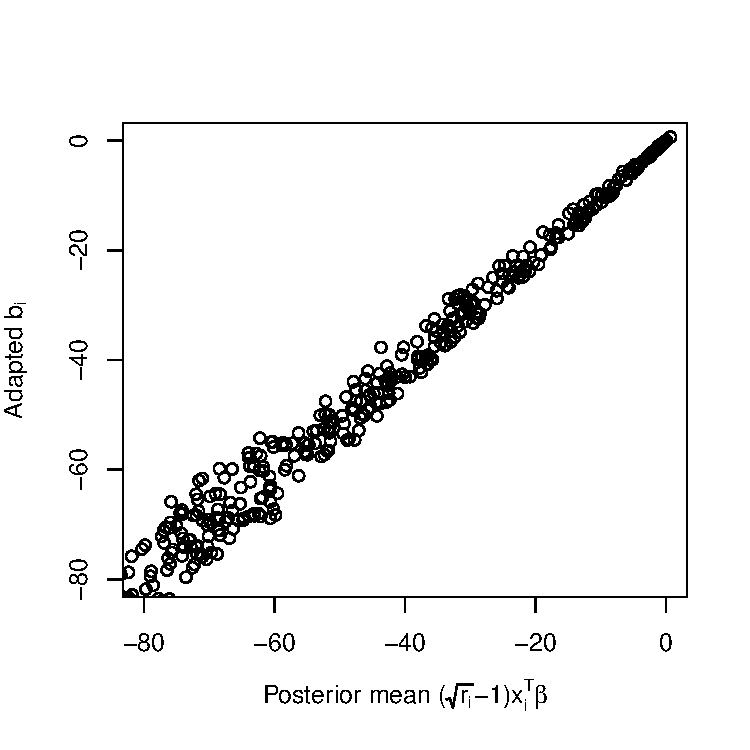
\includegraphics[width=1\textwidth]{probit_cda_b}
  \caption{Numerically optimized $b_i$ in the proposal appearing linear and close to the true bias in $(1-\sqrt{r_i} ) \xbeta$.}
\end{subfigure}
\label{probit_demo}
 \caption{Panel (a) demonstrates in traceplot and panel (b) in autocorrelation about the substantial improvement in CDA by correcting the variance mis-match in probit regression with rare event data, compared with the original \citep{albert1993bayesian} and parameter-expanded methods \citep{liu1999parameter}. Panel (c) shows the degree of the variance increase in $r_i$ (if $r_i=1$: no increase) with respect to the value of $\xbeta$. Panel (d) shows the bias correction term is close to the true bias if no correction were made. }
 \end{figure}
 
\subsubsection{Approximate Method}

The numeric solution presented above is generally applicable. In some cases  if the approximate error is strictly bounded, the algorithm can be further simplified to direct sampling without the Metropolis-Hastings step.

Let $d(\theta, \theta_{r,b})$ be the distance between the two posteriors based on the exact and approximate method. For example, it can be the Kullback-Leibler distance $E\sum_i \{ \log L_{r,b}(y_i | \theta) - \log L(y_i| \theta)\}$. Alternatively, the more loose but useful bound is the norm distance between the first two moments $||\mbox{E}(\theta|y)-\mbox{E}_{r,b}(\theta|y)||$,  $||\mbox{var}(\theta|y)-\mbox{var}_{r,b}(\theta|y)||$. Both criteria would be carefully examined in the next section.

To check if there is a good analytical approximate, the method first proceeds in the same way as the numeric one by increasing the conditional variance and adjusting for correcting bias. Then it starts to differ by examining if the exact bias $f_b(\theta,y_i,r_i)$ can be approximated by a function without $\theta$, at least in some region of $\theta$.

If the approximation function exists, it is used for setting value of $b$ in each step. This leaves one working parameter $r$ to control the approximate error, quantified by the $d(\theta, \theta_{r,b})$. Therefore,  $r$ is used adaptively to bound over the posterior sample $\varTheta^*$ so that $\sup_{\theta \in \varTheta^*} d(\theta, \theta_{r,b})\le \epsilon$.

\begin{algorithm}[H]
		\caption{Variance Adjusting CDA (Approximate)}
		\label{numerical_cda}
		    \begin{algorithmic}
			\State Increase the variance of $\pi(\theta| z,y)$ by changing the parameter in $\pi(z_i |\theta,y_i)$ with $r_i$;
		\State Integrate the modified density to obtain $L_r(y_i|\theta)= \int \pi_r (z_i|\theta) \pi(y_i|z_i,\theta) d z_i$; 
		\State Compare with $L(y_i|\theta)$, include another bias correction parameter $b$ so that $L_{r,b}(y_i|\theta)$ can be equal to $L(y_i|\theta)$ with some $b$ for all $r$.
		\State Derive the analytical form of $f_b(\theta,y_i,r_i)$ so that $L_{r,b={f_b(\theta,y_i,r_i)}}(y_i|\theta)=L(y_i|\theta)$;
		\State Check if $f_b(\theta,y_i,r_i)$ can be approximated by $b_i(y_i,r_i)$ in some region of $\theta$.
		\State Initialize $r_i$ to a large value and $b_i$  for $i=1\ldots n$;
		\State \For{ $step=1\ldots N_{Steps}$ }
		\State Generate individual $z_i$ from $\pi_{r,b}(z_i|\theta, y_i)$;
		\State Generate $\theta$ from $\pi_{r,b}(\theta|z, y)$;
		\State If  $ \sup_{\theta \in \varTheta^*} d(\theta, \theta_{r,b})\le \epsilon$ is not satisfied, update $r_i$ and $b_i$;
		\EndFor
		\end{algorithmic}
\end{algorithm}

We found the analytical approximates exist for a wide range of popular distributions, such as logistic, Poisson log-linear and complementary log-log models. In the following example, we use a logistic regression to illustrate the analytical method.


{\bf Calibration Example 3: Mixed Effects Logistic Regression}\
Consider a mixed effects logistic regression with  $L(y_{ij} |\beta, \sigma^2)\propto \frac{\exp\{ (\xbetaij+\sgamma) y_{ij} \} }{1+ \exp(\xbetaij+\sgamma)}$, where $x_{ij}^T\beta$ is the fixed effect with $\beta$ as the parameter of interest, $\sgamma$ is the group random effect with $\gamma_{i} \stackrel{iid}{\sim} N(0, diag\{ \sigma_l^2\})$ for all $i=1\ldots n_i$. We use prior $\pi(\beta)\propto 1$ and $\pi(\sigma_l^2)=\sigma_l^{-2}$. Based on the Polya-Gamma DA proposed by \cite{polson2013bayesian}, the posterior is sampled from $z_{ij}\sim \mathcal{PG}(1, \xbetaij+\sgamma)$, $\gamma_i \sim \mathcal{N}\{  (\sum_j s_{ij} z_{ij} s_{ij}^T   + diag\{\sigma_l^{-2}\}  )^{-1}   \sum_j  s_{ij}   (y_{ij}-\frac{1}{2} - z_{ij} \xbetaij)  ,  ( \sum_j  s_{ij}  z_{ij} s_{ij}^T   + diag\{\sigma_l^{-2}\}  )^{-1}   \}$, $\sigma_l^{2}\sim \mathcal{IG}(n_i/2, \sum_i \gamma_{il}^2/2)$ and lastly $\beta \sim N\{  (x^T diag\{z_{ij}\}x)^{-1}   x^T  (y-\frac{1}{2} -   vec \{ s_{ij}^T\gamma_i \} z)  ,  (x^T diag\{z_{ij}\}x)^{-1}   \}$. Like the probit regression, slow mixing emerges when $\sum y_{ij}$ is small compared to the total sample size $n$.

CDA adjusts the conditional variance $(x^T diag\{z_{ij}\}x)^{-1} $ by reducing the the value of $z_{ij}$. To achieve this, the original Polya-Gamma distribution is replaced by  $z_{ij}\sim \mathcal{PG}(\frac{1}{r_{ij}}, \xbetaij+s_{ij}^T\gamma_i + b_{ij})$ with $r_{ij} \ge 1$ and $b_{ij}$ as the bias-correction term. The integration leads to $L_{r,b}(y_{ij}|\beta, \sigma^2)\propto \frac{\exp\{ (\xbetaij+s_{ij}^T\gamma_i) y_{ij} \} }{ \{ 1+ \exp(\xbetaij+s_{ij}^T\gamma_i +b_{ij}) \}^{1/r_{ij}} }$. Setting $L_{r,b}(y_{ij}|\beta, \sigma^2)= L(y_{ij}|\beta, \sigma^2)$ yields the exact bias correction term $f_b(\theta,y_{ij},r_{ij}) =  \log [     \{ 1+\exp(\eta_{ij}  ) \}^{r_{ij}} -1    ] - \eta_{ij} = \log\{ r_{ij} + \frac{r_{ij}(r_{ij}-1)}{2!} \exp(\eta_{ij})+ \frac{r_{ij}(r_{ij}-1)(r_{ij}-2)}{3!} \exp(2\eta_{ij}) +\ldots \ \}$ with $\eta_{ij}=\xbetaij+s_{ij}^T\gamma_i$. The last equality suggests when $\exp(\eta_{ij})$ is close to $0$, $f_b(\theta,y_{ij},r_{ij}) $ can be simply approximated by $b_{ij} = \log r_{ij}$. The choice for $r_{ij}$ is discussed in the next section.

The resulting CDA algorithm is then:

\begin{equation}\begin{aligned}
		& z_{ij}\sim \mathcal{PG}(\frac{1}{r_{ij}}, \xbetaij+ \sgamma + \log r_{ij}) \\
	& \gamma_i \sim \mathcal{N}\{  (\sum_j s_{ij} z_{ij} s_{ij}^T   + diag\{\sigma_j^{-2}\}  )^{-1}   \sum_j s_{ij}  \{ y_{ij}-\frac{1}{2 r_{ij}} - z_{ij} (\log r_{ij}+ \xbetaij) \}  ,  (\sum_j s_{ij} z_{ij} s_{ij}^T   + diag\{\sigma_j^{-2}\}  )^{-1}   \}\\
	& \sigma_l^{2}\sim \mathcal{IG}(n/2, \sum_{i} \gamma_{il}^2/2)\\
	& \beta \sim N\{  (x^T diag\{z_{ij}\}x)^{-1}   x^T  \{ y-\frac{1}{2} - z (\log r+ vec \{ s_{ij}^T\gamma_i \})\}  ,  (x^T diag\{z_{ij}\}x)^{-1}   \}
\end{aligned}\end{equation}
	

For illustration, we set $\beta=\{-9,1\}$ as the intercept and the slope to $x_1\sim \mathcal{N}(0,1)$, $n= 10^5$ and $n_i=10^2$, and used $s_{ij} =1$ as the random intercept with variance $\sigma^2 = 0.5$. To ensure identifiability, we fix $\gamma_1=0$. This setting leads to rare positive outcome $\sum y_{ij} = 50 $. The different mixing performances in the original DA and the calibrated one are shown in Figure~\ref{logit_random_mixing}.



\begin{figure}[H]
 % \centering
  \begin{subfigure}[b]{0.49\textwidth}
 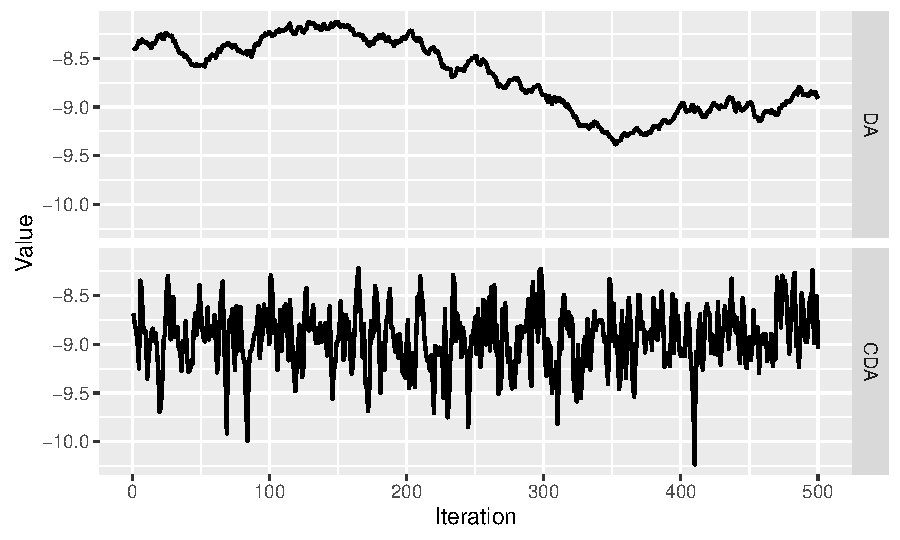
\includegraphics[width=1\textwidth]{logit_random_trace_plot.pdf}
  \caption{Traceplot illustrating mixing performance of the original DA and CDA algorithms in mixed effects logistic regression.}
\end{subfigure}
  \hfill
   \begin{subfigure}[b]{0.49\textwidth}
 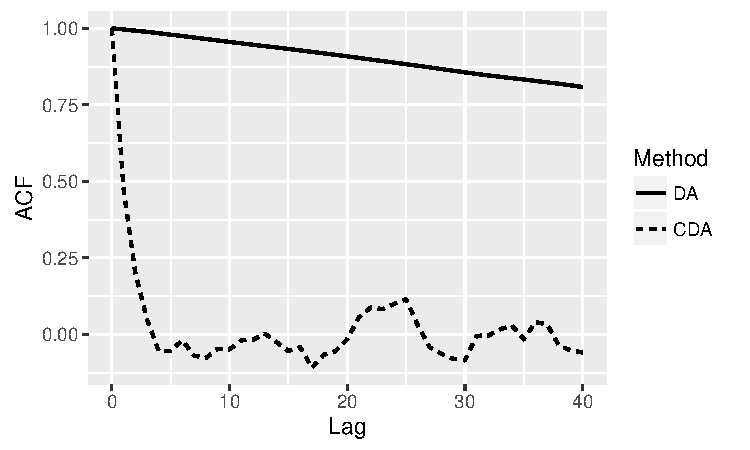
\includegraphics[width=1\textwidth]{logit_random_acf.pdf}
  \caption{Autocorrelation function (ACF) illustrating the large difference between the mixing performance of the original DA and CDA.}
\end{subfigure}
 \caption{Panel (a) demonstrates in traceplot and panel (b) in autocorrelation about the substantial improvement in CDA by correcting the variance mis-match in mixed logistic regression with rare event data, compared with the original \citep{polson2013bayesian}.}
    \label{logit_random_mixing}
 \end{figure}
 
\section{Theory}

\subsection{Mixing Accelaration}

The mixing of Markov chain is related to its geometric convergence rate. Let $\mathcal{P}(\theta,.)$ be the the Markov transition kernel and $\pi(.)$ be its stationary density and $\theta$ be the state in the state space $\varTheta$. The chain is geometrically ergodic if there exist $M: \mathcal{X} \rightarrow [0, \infty)$ and $\rho\in[0,1)$ such that $||\mathcal{P}^k(\theta,.)-\pi(.) ||_{TV} \le M(\theta^{(0)}) \rho^k$, where $||.||_{TV}$ is the total variation distance $|| P_1 -P_2 ||_{TV} = \underset{\mathcal A\in \mathcal F}\sup ||P_1(\mathcal A)-P_2(\mathcal A)||$.

Consider a Hilbert space $L^2(\pi)=\{s(\theta): E\{s(\theta)\}=0, var\{s(\theta)\}<\infty \}$. The forward operator $\bf{F}$ can be defined as ${\bf F}s(\theta)=\int \mathcal{P}(\theta,\theta') s(\theta') d\theta' = E\{ s(\theta') | \theta \}$, whose norm is equal to the maximal correlation between two states $||{\bf F}||=\underset{s(\theta),t(\theta)\in L^2(\pi)}{\sup}\;\mbox{corr}(s(\theta),t(\theta^{'}))$ \citep{liu2008monte}. This norm is directly related to the convergence rate $\rho$: when the chain is reversible with detailed balance (e.g. Metropolis-Hastings), $\lim_{k\rightarrow \infty}||{\bf F}^k||^{1/k}=\rho$; when the chain is non-reversible (e.g. Gibbs sampling), $||{\bf F}||^2$ is equal to the convergence rate of the reversibilized chain \citep{fill1991eigenvalue}.

The two calibrating strategies proposed in the last section reduce the operator norm.

\begin{theorem}
Let ${\bf F}$ and ${\bf F}_{MS}$ be the operators corresponding to the standard DA and the calibrated DA modified with marginalization and sampling (MS), then $||{\bf F}_{MS}||\le ||{\bf F}||$.
\end{theorem}


\begin{theorem}
Let ${\bf F}$ and ${\bf F}_{IV}$ be the operators corresponding to the standard DA and the calibrated DA modified with increased variance (IV). If the relative difference in marginal variance $\frac{|\mbox{var}\{s(\theta)|y  \} - \mbox{var}_{IV}\{s(\theta)|y\} |}{\mbox{var}\{s(\theta)|y \} }\le \epsilon$ and the variance increase $\frac{ var_{IV}\{ \theta|z,y\}}{ var\{ \theta|z,y\}} \ge (1+\epsilon) $, then $||{\bf F}_{IV}||\le ||{\bf F}||$.
\end{theorem}

\subsection{Error Control in Approximate CDA}

For approximate CDA with increased variance, the error needs to be carefully controlled. One can bound the total variation distance $||{P}-{P}_{r,b} ||_{TV}$, where ${P}$ and ${P}_{r,b}$ are the measures for the stationary distributions corresponding to the exact and approximate algorithms. From this bound, one can control the errors of the posterior mean and variance.

\begin{theorem}
Let $\theta$ be the $p$-element vector of $\{\theta_j\}_{j=1\ldots p}$.
If the total variation distance between the two measures defined as above is small $||{P}- {P}_{r,b} ||_{TV}\le \epsilon_1$, $\pi(\theta|y)$ and $\pi_{r,b}(\theta|y)$ have the tail square integral negligible when $|\theta|>M$,  $E \theta_j^2 {1}_{|\theta_j|>M}\le \epsilon_2$ and $E_{r} \theta_j^2 {1}_{|\theta_j|>M}\le \epsilon_2$. Let $M$ be large enough so that $\epsilon_2=o(\epsilon_1)$, then the approximation errors between the first two central moments of $\theta_j$ have:
$$|\mbox{E}(\theta_j|y)-\mbox{E}_{r,b}(\theta_j|y)|\le 2M\epsilon_1+ o(\epsilon_1),$$
$$|\mbox{var}(\theta_j|y)-\mbox{var}_{r,b}(\theta_j|y)|\le 6M^2\epsilon_1+o(\epsilon_1).$$
\end{theorem}
 
 \begin{remark}
 	The assumption on the tail is guaranteed by the existence of the second moment, which implies uniform integrablity. The bound on the variance difference is particularly useful in guaranteeing the average increased conditional variable could at most exceed the target variance by a small error $E^z\mbox{var}_{r,b}(\theta_j|z,y)\le\mbox{var}(\theta_j|y)+\epsilon$, with $\epsilon$ as a polynomial function of $\epsilon_1$ defined as above.
 \end{remark}
 
 The approximation error for the covariance can be similarly bounded:

\begin{corollary}
If $||{P}- {P}_{r,b} ||_{TV}\le \epsilon_1$ and $\pi(\theta|y)$ and $\pi_{r,b}(\theta|y)$, $E \theta_j^2 {1}_{|\theta_j|>M_j}\le \epsilon_2$ and $E_{r,b} \theta_j^2 {1}_{|\theta_j|>M_j}\le \epsilon_2$ for all $j$.  Let $M_j$ be large enough so that $\epsilon_2=o(\epsilon_1)$, then the approximation error between the covariances:
$$|\mbox{cov}(\theta_{j_1},\theta_{j_2}|y)-\mbox{cov}_{r,b}(\theta_{j_1},\theta_{j_2}|y)|\le 6M_{j_1}M_{j_2}\epsilon_1+o(\epsilon_1 ).$$
\end{corollary}

As a special case, we consider in generalized linear model where the total likelihood can be broken into $L(y| B\theta) = \prod  L( y_{i}| B_i^T \theta)$. Here the linear part $B_i^T \theta$ is set in general sense, which could be the combination of both fixed and random effects. Rather than controlling the total distance between $L(y| B\theta)$ and $L_{r,b}(y| B\theta)$, under some  mild conditions of the predictor matrix $B$, one can focus on bounding the maximum error in individual $B_i^T \theta$, based on $ L( y_{i}| B_i^T \theta)$ over $i=1\ldots n$.

\begin{theorem}
If $B^TB$ is full rank and let $B^{-}:=(B^TB)^{-1}B^T$, the following inequalities hold:\\
$$||{E}\theta-{E}\theta_{r,b}||_1 \le ||B^{-}||_1 ||{E}B\theta- {E}B\theta_{r,b}||_\infty$$
$$||\mbox{cov}\theta-\mbox{cov}\theta_{r,b}||_1 \le ||B^{-}||_1 ||B^{-}||_\infty ||\mbox{cov} B\theta- \mbox{cov}B\theta_{r,b}||_\infty$$
\end{theorem}

 \begin{remark}
One reason for using these inequalities is that the norms $||B^{-}||_1$ and $||B^{-}||_\infty$ are usually quite small compared to $n$.  For example, a well-conditioned matrix has $||B^{-}||_\infty\approx p/n$ and $||B^{-}||_1\approx p$.
 \end{remark}

We return to examine the approximate CDA for mixed effects logistic regression, and determined the suitable range for $r_{ij}$.

{\bf Calibration Example 3 (continued): Mixed Effects Logistic Regression}

In the CDA for mixed effects logistic regression, the effective approximate likelihood is $L_{r,b}(y_{ij}|\eta_{ij}) = \frac{\Gamma(1/r_{ij}+1)}{\Gamma(y_{ij}+1)\Gamma(1/r_{ij}-y_{ij}+1)}\frac{\exp (\eta_{ij}+ \log r_{ij})^ {y_{ij}}}{\{1+\exp (\eta_{ij}+ \log r_{ij})\}^{1/r_{ij}}}$. The distance between the approximate and the true likelihoods for each $i$ has $|| { P_{r,b}(y_{ij}|\eta_{ij}) } - {P(y_{ij}|\eta_{ij})} )||_{TV} \le   \{   \frac{\sqrt{r_{ij}-1}  \exp(\eta_{ij})}{2} \} 1 \{\eta_{ij}< - \log r_{ij} \le 0 \}$. The tail square integral $E \eta^2_i 1(|\eta_{ij}|>M) = O\{ M^2 \exp(-M)\}$. Given a maximally tolerable approximation error $\epsilon=0.01$, the calculation leads to  $r_{ij} \le  [\{\frac{10^{-3} }{\exp(\eta_{ij})}\}^2  \wedge {\exp(-\eta_{ij})} ]  \vee 1$. This suggests to apply calibration when $\eta_{ij}< -6.9$ approximately, which is consistent with the rare event scenario.

\subsection{Ergodicity}

The conditions for ergodicity should be met for Markov chains. In the CDA based on marginalization, obviously as long the original chain is ergodic, so is the marginalized chain is, due to its smaller norm of the forward operator. For the CDA based on variance increase, the adaption of the working parameters could influence the ergodicity. In the numeric method, we stop adaption after the tuning period; in the approximate solution, we rely on the the results from \cite{roberts2007coupling} that an adaptive Markov chain is uniformly ergodic, if (i) the transition kernel corresponding to each $r$ is uniformly ergodicity (simultaneous convergence) and (ii) the total variation distance between kernels in two adjacent steps converges to $0$ in probability (diminishing adaptation).

The first condition is simple to achieve since the approximation does not alter the distribution of the transition kernel but only with different parameterization, the condition can be met with only slight modification. For the diminishing adaptation, since $r$ is adapted so that $\sup_{\theta \in \varTheta^*} d(\theta, \theta_{r,b})\le \epsilon$ over the posterior sample $\varTheta^*$, the suitable $r$ could be the extreme function of the posterior $\theta$. When it is true, the convergence of the extreme function in probability leads to the convergence of the transition kernel.

{\bf Calibration Example 3 (continued): Mixed Effects Logistic Regression}

In the CDA with mixed effects logistic regression, we set $r_{ij} =  1 \vee \underset{\eta_{ij}: \theta\in \varTheta^*}{\inf}[\{\frac{10^{-3} }{\exp(\eta_{ij})}\}^2  \wedge {\exp(-\eta_{ij})} ]   $, which is related to the maximum of $\eta_{ij}=\xbeta+s_{ij}\gamma_i$ if $\eta_{ij}<0$. With finite posterior variance of $\beta$ and $\gamma_i$, the value is convergent in probability via Chebyshev's inequality. The diminishing adaption for the numeric example is shown in Figure~\ref{diminishing_adapt}.

 \begin{figure}[H]
 \centering
 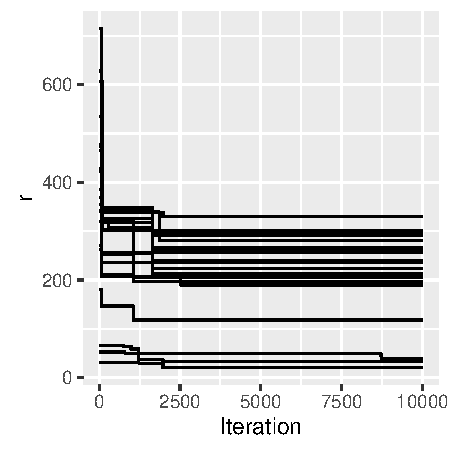
\includegraphics[width=0.3\textwidth]{r_adaptation.pdf}
  \caption{The diminishing adaptation of the working parameter $r_{ij}$ in mixed effects logistic regression.}
  \label{diminishing_adapt}
 \end{figure}

\section{Real Data Application: Poisson Regression for Online Advertisement Tracking}

We now apply CDA to a large data application in online advertisement tracking. The dataset contains the click-through count between pairs of website. There are $n=59,792$ originating websites, where the advertisement is displayed, and $96$ different target websites where the link points to. The training data is collected during a two-week period, the a non-overlapping set is collected during another two-week time for validation. For a given website, it is of commercial interests to predict the traffic from each originating one $y_i$, using the information from the other $p=95$ websites $x_{i,1},\ldots, x_{i,95}$. Therefore, this leads to a count data regression.

A significant proportion of the originating websites do not produce traffic to the target one. The outcome data are saturated with zeros and  only $4.5\%$ contain positive counts. For this scenario, Poisson log-linear model  $y_i\sim Poisson\{\exp(x_i^T\beta)\}$  is known for slow mixing, due to the same variance mis-match caused by the rare positive outcomes. The predictor-based zero-inflated Poisson such as $y_i\sim \pi_i\{ g(X_i^T\beta_1)\}  1(y_i=0)+ \{ 1-\pi_i(g(X_i^T\beta_1)) \} Poisson\{\exp (X_i^T \beta_2)\}$ does not alleviate the mixing issue, on the contrary,  mixing is even slower because of the high correlation of $\pi_i$ and those with Poisson mean close to $0$.

Rather, we consider calibrating the simpler model  $y_i\sim Poisson\{\exp(\beta_0+ \sum_j x_{i,j}\beta_j)\}$ directly. Provided the mixing performance is satisfying, the intercept $\beta_0$ would be large and negative with significant uncertainty; at the same time, a small proportion can deviate from mean $0$ based on their distinctively large predictors. This simple and tractable model would achieve the same goal as the predictor-based zero-inflated model.

{\bf Calibration Example 4: Poisson Log-Linear Regression with Zero-Inflated Data}

We first derive an approximate CDA for Poisson log-linear regression. All the existing data augmentation methods for Poisson log-linear involve approximation. For Poisson with large mean, normal approximation works reasonably well; for small ones, \cite{zhou2012lognormal}  used negative binomial $\mathcal{NB}\{ \alpha,\frac{\exp(\xbetaij)}{\exp(\xbetaij)+\alpha}\}$ with large $\alpha$ to connect to the Polya-Gamma augmentation. Here, we utilize a simpler limit form $L(y_i|\xbeta)=\frac{ \exp(y_i \xbeta)}{\exp\{\exp(\xbeta)\}y!} =\lim_{\lambda\rightarrow\infty}\frac{\exp(y_i \xbeta)}{\{1+ \exp(\xbeta)/\lambda\}^{\lambda}y!}$. Using a flat prior on $\beta$, the Polya-Gamma augmentation leads to approximate posterior sampling $z_i \sim \mathcal{PG}\left\{\lambda, \xbeta -\log \lambda\right\}$ and $\mathcal{N}\big[ (x^T diag\{z_i\} x )^{-1} (x^T  \big \{ y - \lambda/2 + z \log \lambda \big\} ),(x^T diag\{z_i\} x )^{-1} \big]$, with large $\lambda$.

Without calibration, the mixing is slow as the conditional variance for $\beta$ is quite small, due to the large $z_i$ caused in large $\lambda$ approximation. To calibrate, we replace the above Polya-Gamma with $z_i \sim \mathcal{PG} ( \frac{1}{r_i}, \xbeta + b_i )$ and compare the integrated form with the Poisson density. This leads to the exact bias correction $f_b(\theta,y_{i},r_{i})= \log \frac{\exp\{\exp(\xbeta)r_i\}-1}{\exp(\xbeta)}= \log \{ r_i+ \frac{r_i^2}{2}\exp(\xbeta)+ \frac{r_i^3}{3!}  \exp(2\xbeta)+\ldots \} $, which can be approximated b  $b_i = \log r_i$ when $\exp(\xbeta)$ is close to $0$. When $r_i\rightarrow 0$, the bias is eliminated.

The resulting CDA is:


\begin{equation}\begin{aligned}
		& z_{i}\sim \mathcal{PG}(\frac{1}{r_{i}}, \xbetaij+ \log r_{i}) \\
	& \beta \sim N\{  (x^T diag\{z_{i}\}x)^{-1}   x^T (y-\frac{1}{2 r} + z \log r)  ,  (x^T diag\{z_{i}\}x)^{-1}   \}
\end{aligned}\end{equation}

The effective approximate likelihood is $L_{r,b} (y_i| \xbeta) =\frac{\Gamma(1/r_i+1)}{\Gamma(1/r_i-y_i+1)\Gamma(y_i+1)}\frac{\exp ( \xbeta+\log r_i)^y_i}{\{1+ \exp ( \xbeta +\log r_i)\}^{1/r_i}}$ with $r_i< 1/(y_i -1)$. The total variation distance $||L (y_i| \xbeta) - L_{r,b} (y_i| \xbeta)||_{TV}\le \frac{\sqrt r_i }{2}\exp (\xbeta)$. The bound on the tail square integral is provided in the appendix. Given a maximally tolerable approximation error $\epsilon=0.01$, the calculation leads to  $r_{i} = \underset{\theta \in \varTheta^*}{\inf}  \{\frac{10^{-3.5} }{\exp(\xbeta)}\}^2   $.

We ran the uncalibrated DA with large $\lambda=10,000$ and CDA for posterior computation. We started all three algorithms by assigning the same initial value $(x^Tx)^{-1}(x^T \log( y+1))$ to ${\beta}$. We ran each algorithm for $4000$ steps and used the last $1,000$ as the posterior sample.

The mixing of DA and CDA is compared by traceplots and autocorrelation plots in Figure~\ref{data_poisson}. DA shows slow mixing for several parameters (Figure\ref{acf_poi_da}), including the important intercept estimate $\beta_0$ (first plot in Figure\ref{traceplot_poi_da}). In contrast, CDA performs extremely very well in terms of mixing (Figure\ref{acf_poi_ada}). This is shown by the low autocorrelation in all of the $96$ parameters. 

 \begin{figure}[H]
 % \centering
   \begin{subfigure}[b]{0.45\textwidth}
 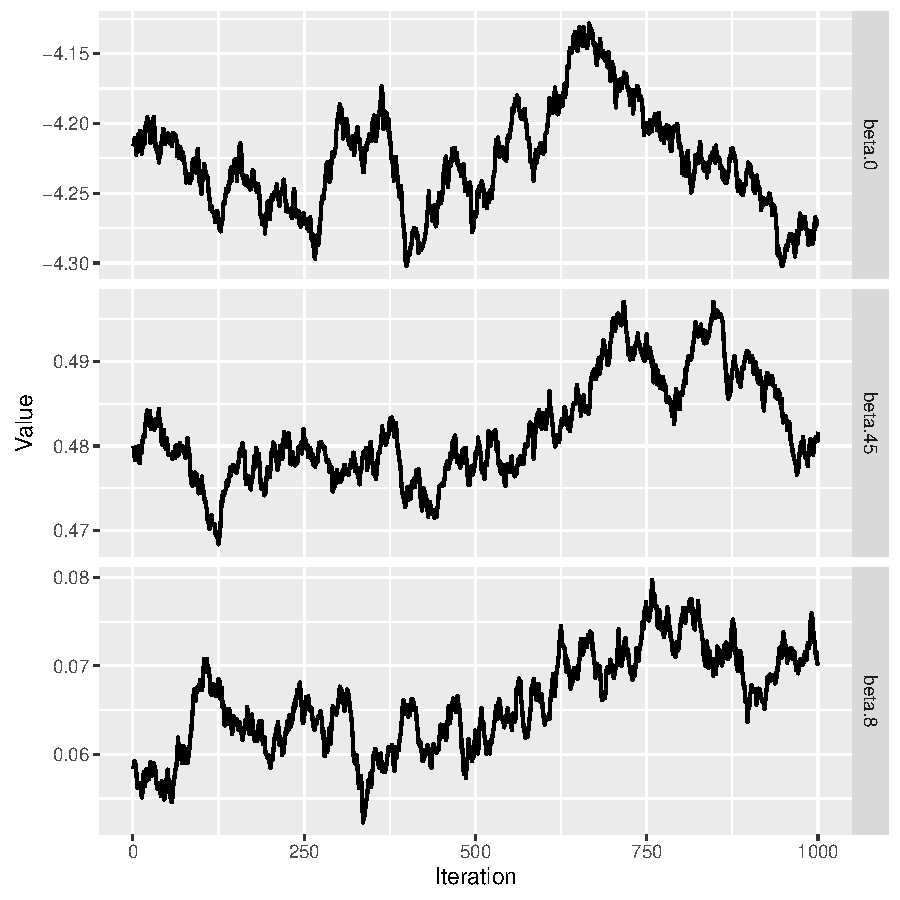
\includegraphics[width=1\textwidth]{traceplot_poisson_da.pdf}
 \caption{Trace plots of three parameters from DA.}
  \label{traceplot_poi_da}
 \end{subfigure}
  \hfill 
 \begin{subfigure}[b]{0.45\textwidth}
 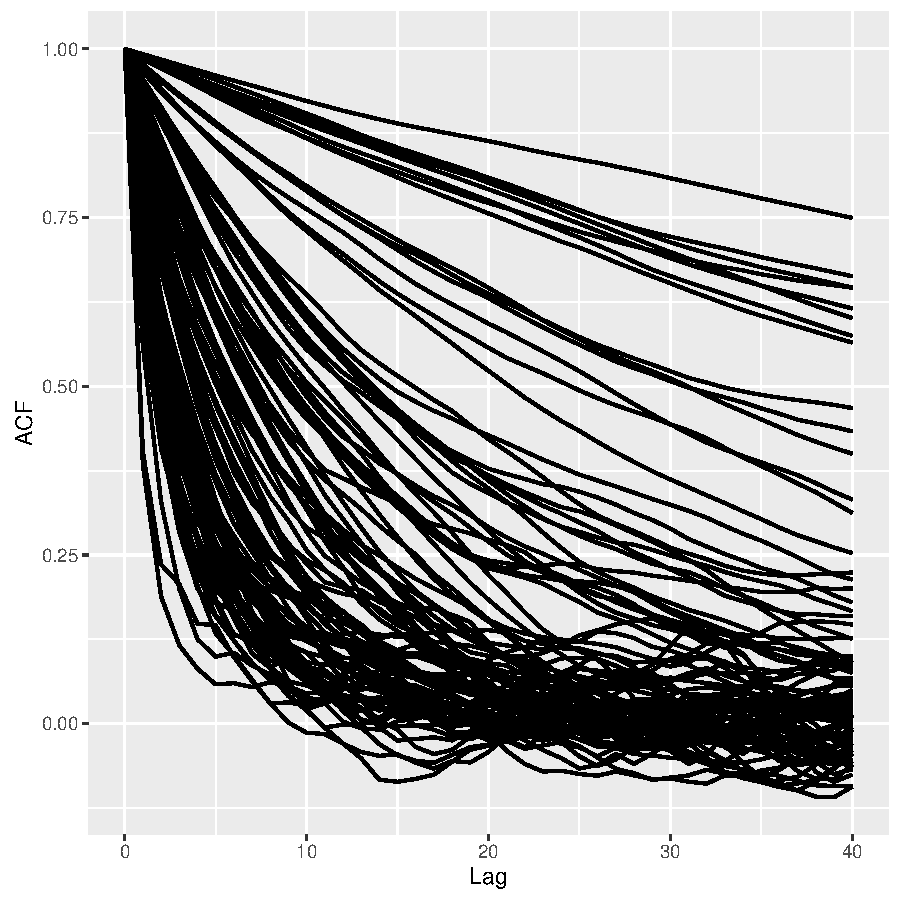
\includegraphics[width=1\textwidth]{poisson_da_acf.pdf}
 \caption{Autocorrelation of all the 96 $\beta$'s from DA.}
   \label{acf_poi_da}
 \end{subfigure} 
  \begin{subfigure}[b]{0.45\textwidth}
 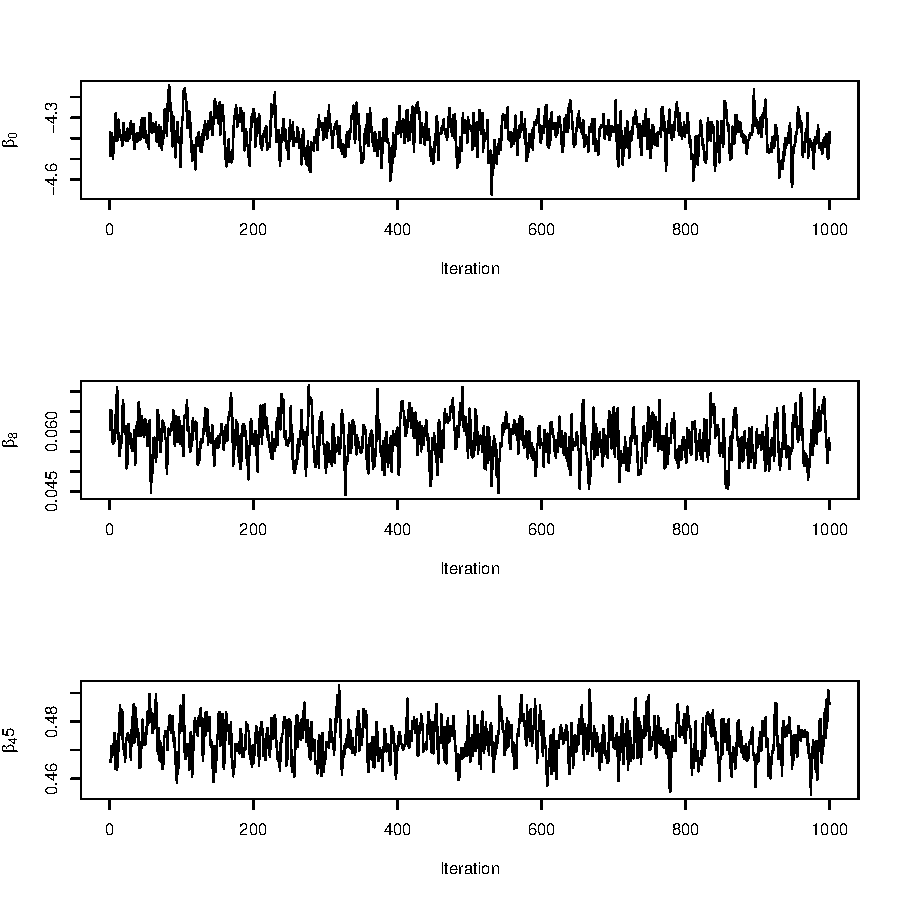
\includegraphics[width=1\textwidth]{traceplot_poisson_ada.pdf}
 \caption{Trace plots of three parameters from CDA.}
  \label{traceplot_poi_ada}
 \end{subfigure}
  \hfill 
 \begin{subfigure}[b]{0.45\textwidth}
 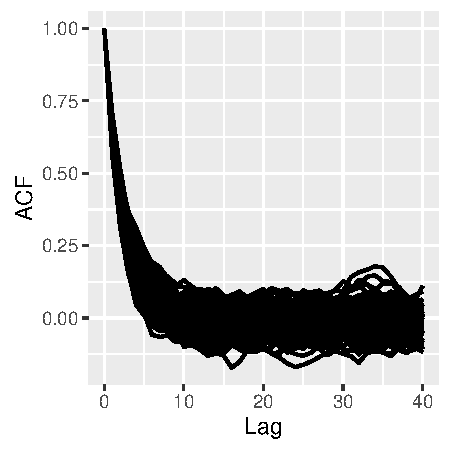
\includegraphics[width=1\textwidth]{poisson_ada_acf.pdf}
 \caption{Autocorrelation of all the 96 $\beta$'s from CDA.}
   \label{acf_poi_ada}
 \end{subfigure}
 \caption{Compared with DA, CDA produces much faster mixing posterior sample.}
 \label{data_poisson}
 \end{figure}



We list the parameter estimates and fit statistics in Table~\ref{table:Poisson}. For simplicity, we include the posterior mean and standard deviation for the intercept $\beta_0$ and the sum of slopes $\sum_{j=1}^{95} \beta_j$. To assess goodness-of-fit, we also evaluate root-mean-squared error $RMSE= \sqrt{ \sum_{i=1}^n  (y_i-\mu_i)^2/n}$ and the deviance $D=2\sum_{i=1}^n \{ y_i \log(y_i/\mu_i) -(y_i-\mu_i)\}$, with $\mu_i=\exp( x_i{\hat\beta})$ and ${\hat\beta}$ the posterior mean. For prediction performance, we use the testing dataset collected $\{ y_{new},  x_{new}\}$ on the same websites and $\tilde y_{i,new}=\exp( x_{i,new}{\hat\beta})$ as the estimator. We evaluate the cross-validation RMSE between $y_{i,new}$ and $\tilde y_{i,new}$.

As expected, the estimate for $\beta_0$ is quite negative, which is captured by the point estimates of both DA and CDA. However, DA severely underestimates the variance of the intercept. The estimates for the $95$ covariates also differ greatly from CDA. Obviously, the poor mixing causes the Markov chain in DA to be trapped in a suboptimal state, whereas CDA performs exceptionally well in fit statistics and the validation error that is almost $4$ times lower. More details in comparing the fitted and prediction are provided in the appendix.

To verify the result, we additionally ran Hamiltonian Monte Carlo (HMC) as the reference. HMC is known for its good mixing properties but very costly evaluation. The result of CDA agrees very well with HMC in both the posterior mean and standard deviation on all the $95$ slope parameters (see appendix for comparison plots). For HMC, it requires significant tuning to reach ideal step size and length for proposal; while CDA only require one additional  step in generating the latent variable. Therefore, CDA is significantly more efficient than HMC and took only $1/10$ of the computing time.


\begin{table}[H]
\centering
\begin{tabular}{|l |r |r| r| r |} 
 \hline
                          & DA & CDA & HMC\\
 [0.5ex]
 \hline
$\beta_0$                         & -4.21 (0.042)& -4.38 (0.075) & -4.47 (0.071) \\
$\sum_{j=1}^{95} \beta_j$         & -0.11 (0.063)& 0.69 (0.053)  & 0.70 (0.055)  \\
RMSE                              & 32.86        & 5.06          & 4.88\\
D                                 & 182127.7     & 107076.9      & 106791.3\\
CV-RMSE                           & 32.01        & 8.61          & 8.28\\
Steps to Converge                 & 2000         & 50            & 500 \\
Computing Time (per 2,000 steps)  & 50 mins       & 51 mins        & 600 mins\\
 \hline
\end{tabular}
\caption{Performance of DA, CDA and HMC in Poisson log-linear regression with online advertisement tracking data. Posterior estimates for the intercept and sum-of-slopes are shown. The CDA shows much better fit statistics such as root-mean-squared error (RMSE) and deviance (D). In cross-validation (CV-RMSE), the CDA outperforms DA as well. The CDA converges much more rapidly than DA. Compared to the reference, CDA agrees with the HMC very well but takes significantly less time.}
\label{table:Poisson}
\end{table}


\section{Discussion}

The slow mixing is a severe problem that prevents data augmentation based MCMC from be applicable on large dataset. With data size increases and become complex, it is common for the parameters to deviate from the area that has reasonable mixing performance. As we show in the previous example, it does not only lead to an un-manageable increase in the computational time, but also could cause Markov chain to be trapped in the suboptimal state.  Therefore, it is necessary to address this issue if we want to keep data augmentation useful in large data.

In this article, we propose a general class of solutions that calibrates this issue. Based on the data augmentation factorization, CDA either integrates out the parameter or increases its conditional variance, so that the step size is adjusted onto the same order of the marginal variance. 

In the data application, we use Hamiltonian Monte Carlo as a good reference for parameter estimation. Here we draw a comparison between the variance increased CDA and HMC.  The ideal Markov chain kernel would be to propose, based on the current state, a state that is as uncorrelated as possible; in the meantime, with high acceptance probability to move to the new state. The HMC utilizes numerical simulation of Hamiltonian dynamics and a long walk to generate such a proposal. In contrast, the CDA directly utilizes the original density but with an increased conditional variance to reduce the correlation. The  short distance between the proposal and current likelihood  enables a good acceptance rate as well. The difference between the two is that the HMC is computationally costly since it relies on evaluation of gradients and multiple Hamiltonian steps for each proposal; whereas CDA does not use gradient but only one-step update, which is almost at the same low cost as the conventional DA method. 


\bibliography{reference}
\bibliographystyle{plainnat}


\section{Appendix}

\subsection{Proof of Theorems}

\subsubsection{Proof of Theorem 1:}


Let $\theta=\{\theta_1, \theta_2\}$ be the parameters that are divided into two parts. Let $\theta'$ and $z'$ be the parameters and latent variables in the last iteration. Omitting $y$ for the ease of notation, the square of maximal correlation can be represented as $||{\bf F}||^2=\underset{s(\theta,z),t(\theta,z)\in L^2(\pi)}{\sup}\;\mbox{corr}\{s(\theta,z),t(\theta^{'},z')\}^2
= \underset{s(\theta,z)\in L^2(\pi)}{\sup}\; \frac{\mbox{var} [ E \{ s(\theta,z)|\theta^{'},z'\}]}{\mbox{var}\{s(\theta,z) \} }$.

The original DA samples in the order of $ \{\theta'_1, \theta'_2\} \rightarrow z' \rightarrow \{\theta_1, \theta_2\}\rightarrow z$, with $ \mbox{var} [ E \{ s(\theta,z)|\theta^{'},z'\}] =  \mbox{var} [ E \{ s(\theta_1, \theta_2,z)|\theta^{'}_1,\theta^{'}_2,z'\}] $. The marginalization and sampling based CDA samples  in the order of $ \theta'_2 \rightarrow z' \rightarrow \theta_2\rightarrow z$, followed by $z' \rightarrow \theta'_1$ and  $z \rightarrow \theta_1$ with $ \mbox{var} [ E \{ s(\theta,z)|\theta^{'},z'\}] =  \mbox{var} [ E \{ s(\theta_1, \theta_2,z)|\theta^{'}_1,\theta^{'}_2,z'\}] = \mbox{var} [ E \{ s(\theta_1, \theta_2,z)|\theta^{'}_2,z'\}]$.

For better clarity, let $E_{X}$ denote the integration over $P(dX)$. 

\begin{equation}
\begin{aligned}
 \mbox{var} [ E \{ s(\theta_1, \theta_2,z)|\theta^{'}_2,z'\}]  & = E_{\theta^{'}_2,z'}  [ E_{\theta_1, \theta_2,z}\{ s(\theta_1, \theta_2,z)|\theta^{'}_2,z' \} ]^2 -  (E_{\theta^{'}_2,z'}   [ E_{\theta_1, \theta_2,z}\{ s(\theta_1, \theta_2,z)|\theta^{'}_2,z' \} ])^2  \\
 & = E_{\theta^{'}_2,z'}   [ E_{\theta'_1}E_{\theta_1, \theta_2,z} \{ s(\theta_1, \theta_2,z)|\theta'_1, \theta^{'}_2,z' \} ]^2 - (E_{\theta^{'}_1,\theta^{'}_2,z'}   [ E_{\theta_1, \theta_2,z} \{ s(\theta_1, \theta_2,z)|\theta^{'}_1,\theta^{'}_2,z' \} ])^2 \\
& \le  E_{\theta^{'}_2,z'}  E_{\theta'_1} [ E_{\theta_1, \theta_2,z} \{ s(\theta_1, \theta_2,z)|\theta'_1, \theta^{'}_2,z' \} ]^2 - (E_{\theta^{'}_1,\theta^{'}_2,z'}   [ E_{\theta_1, \theta_2,z} \{ s(\theta_1, \theta_2,z)|\theta^{'}_1,\theta^{'}_2,z' \} ])^2\\
& =  \mbox{var}  [E \{ s(\theta_1, \theta_2,z)|\theta^{'}_1,\theta^{'}_2,z'\}] 
\end{aligned}
\end{equation}

This completes the proof.


\subsubsection{Proof of Theorem 2:}

Both DA and the variance increase CDA sample in the order of  $\theta' \rightarrow z' \rightarrow \theta \rightarrow z$. Omitting $y$ for the ease of notation, by Lemma 4 of \cite{liu1994collapsed}, $\underset{s(\theta)\in L^2(\pi)}{\sup}\; \frac{\mbox{var} [ E \{ s(\theta,z)|\theta^{'},z'\}]}{\mbox{var}\{s(\theta,z) \} } = \underset{s(\theta)\in L^2(\pi)}{\sup}\; \frac{\mbox{var} [ E \{ s(\theta)|z'\}]}{\mbox{var}\{s(\theta) \} }$.

As  $\frac{ var_{IV}\{ \theta|z\}}{ var\{ \theta | z\}} \ge (1+\epsilon) $ leads to  $E    [var_{IV}\{ \theta|z\}] \ge (1+\epsilon) E[var\{ \theta|z\}]$, $\frac{|\mbox{var}\{s(\theta)  \} - \mbox{var}_{IV}\{s(\theta)\}| }{\mbox{var}\{s(\theta) \} }\le \epsilon$ leads to $ \mbox{var}_{IV}\{s(\theta)  \} \le (1+\epsilon)  \mbox{var}\{s(\theta) \} $.

\begin{equation}
\begin{aligned}
1- \frac{E    [var_{IV}\{ \theta|z\}]}{\mbox{var}_{IV}\{s(\theta) \}} \le 1- \frac{ (1+\epsilon) E[var\{ \theta|z\}]}{(1+\epsilon)  \mbox{var}\{s(\theta) \} }
\end{aligned}
\end{equation}

Using $\mbox{var} \{ s(\theta)\} = E    [var\{ s(\theta)|z\}] + var    [E\{ s(\theta)|z\}]$ and taking supremum on both sides complete the proof.


\subsubsection{Proof of Theorem 3:}

Without loss of generality, take $M\ge 1$, then $E |\theta_j| {1}_{|\theta_j|>M}\le E \theta_j^2 {1}_{|\theta_j|>M}\le \epsilon_2$.

\begin{equation}
\begin{aligned}
|E (\theta_j |y)-E_{r,b} (\theta_j |y)| & = \int  | \theta_j \pi(\theta_j | y) -  \theta_j\pi_{r,b}(\theta_j|y)| d\theta_j  \\
& \le \int  | \theta_j| |\pi(\theta_j | y) - \pi_{r,b}(\theta_j|y)| d\theta_j  \\
& =   \int  1(|\theta_j|\le M) | \theta_j|\cdot |\pi(\theta_j | y) - \pi_{r,b}(\theta_j|y)| d\theta_j  +  \int 1(|\theta_j|>M) | \theta_j| |\pi(\theta_j | y) - \pi_{r,b}(\theta_j|y)| d\theta_j  \\
& \le M   \int   |\pi(\theta_j | y) - \pi_{r,b}(\theta_j|y)| d\theta_j  + \int 1(|\theta_j|>M) | \theta_j| \pi(\theta_j | y) d\theta_j +  \int 1(|\theta_j|>M) | \theta_j| \pi_{r,b}(\theta_j|y) d\theta_j  \\
& \le 2M\epsilon_1 + 2\epsilon_2 \\
& = 2M\epsilon_1 + o(\epsilon_1),
\end{aligned}
\end{equation}
where triangle inequality and the definition of total variation distance are used.



\begin{equation}
\begin{aligned}
|\mbox{var} (\theta_j |y)-\mbox{var}_{r,b} (\theta_j |y)| & = | [E (\theta^2_j |y)- \{ E(\theta_j |y)\}^2] - [ E_{r,b} (\theta^2_j |y)-\{ E_{r,b} (\theta_j |y)\}^2 ]|\\
& \le | E (\theta^2_j |y)-  [ E_{r,b} (\theta^2_j |y) ] |+ | \{ E(\theta_j |y)\}^2 -\{ E_{r,b} (\theta_j |y)\}^2 ]|\\
& \le 2M^2 \epsilon_1 + 2\epsilon_2 + | \{ E(\theta_j |y)\} -\{ E_{r,b} (\theta_j |y)\} ]| \cdot | \{ E(\theta_j |y)\}+\{ E_{r,b} (\theta_j |y)\}]| \\
& \le 2M^2 \epsilon_1 + 2\epsilon_2 +  (2M\epsilon_1 + 2\epsilon_2) \{  2 E(\theta_j |y) + 2M\epsilon_1 + 2\epsilon_2 \} \\
& \le 2M^2 \epsilon_1 + 2\epsilon_2 +  (2M\epsilon_1 + 2\epsilon_2) \{  2 M+ 2\epsilon_2 + 2M\epsilon_1 + 2\epsilon_2 \} \\
& = 6M^2\epsilon_1 + o(\epsilon_1).
\end{aligned}
\end{equation}


To prove Corollary 1, using Cauchy-Schwarz inequality $ \{  E\theta_{j_1}\theta_{j_2} 1(\theta_{j_1}>M_{j_1} )  1(\theta_{j_2}>M_{j_2} )    \}^2 \le   E\theta^2_{j_1}1(\theta_{j_1}>M_{j_1} )  E \theta^2_{j_2} 1(\theta_{j_1}>M_{j_2} )   =\epsilon^2_2$. Following the similar proof for variance, it can be derived that:

$$|\mbox{cov}(\theta_{j_1},\theta_{j_2}|y)-\mbox{cov}_{r,b}(\theta_{j_1},\theta_{j_2}|y)|\le 6M_{j_1}M_{j_2}\epsilon_1+o(\epsilon_1 ).$$

\subsubsection{Proof of Theorem 4:}

Since $\theta= B^{-} B\theta$, $\mbox{cov} B\theta= B^{-}  \mbox{cov} B\theta B^{-T} $, applying H\"older's inequality:

$$||{E}\theta-{E}\theta_{r,b}||_1 \le ||B^{-}||_1 ||{E}B\theta- {E}B\theta_{r,b}||_\infty$$
$$||\mbox{cov}\theta-\mbox{cov}\theta_{r,b}||_1 \le  ||B^{-}||_\infty ||B^{-}\mbox{cov} B\theta- B^{-}\mbox{cov}B\theta_{r,b}||_1 \le ||B^{-}||_1 ||B^{-}||_\infty ||\mbox{cov} B\theta- \mbox{cov}B\theta_{r,b}||_\infty$$

\subsection{Approximation Error in Logistic Regression}

For better clarity, we renumber the double index $ij$ using single index $i$.

\subsubsection{Total Variation Distance}

The individual Kullback-Leibler distance:

\begin{equation}
\begin{aligned}
KL\{ { L_{r,b}(y_i|\eta_{i}) } || {L(y_i|\eta_{i})} \}& =\mbox{E}\log \frac{\Gamma(1/r_i+1) r_i^{y_i}  /\Gamma(1/r_i -y_i+1)  }{\Gamma(2) /\Gamma(2 -y_i)  } + \log \frac{ 1+\exp(\eta_{i})}{ \{1+\exp(\eta_{i})r_i\}^{1/r_i}}\\
& =\log\{1+ \exp ( \eta_{i})\}   - 1/r \log\{1+ r\exp ( \eta_{i})\}\\
& \le   \{   (r_i-1) \frac{ \exp(2\eta_{i})}{2} \}  1\{\exp(\eta_{i})< 1/r_i\} + \log \frac{ 1+\exp(\eta_{i})}{ \{1+\exp(\eta_{i})r_i\}^{1/r_i}}  1\{\exp(\eta_{i})\ge 1/r_i\} \\
%& \le   \frac{r_i-1}{2 r_i^2}  1\{r_i <\exp(-\eta_{i}) \} + \log \frac{ 1+\exp(\eta_{i})}{ \{1+\exp(\eta_{i})r_i\}^{1/r_i}}  1\{ \eta_{i} \ge -\log r_i\}.
\label{KL_logit}
\end{aligned}
\end{equation}


With adaptive $r_i=1$ if $\eta_{i}\ge -\log r_i$ and Pinsker's inequality,

$$||P_{r,b}(y_i|\eta_{i}) - P(y_i|\eta_{i})||_{TV} \le   \{   \frac{\sqrt{r_{i}-1}  \exp(\eta_{i})}{2} \} 1 \{\eta_{i}< - \log r_{i} \le 0 \}$$

\subsubsection{Tail Integral}

Consider each likelihood $L(y_i|p_i) = p^y_i (1-p)^{1-y_i}$ with $p_i=\frac{\exp(\eta_{i})}{1+\exp(\eta_{i})}$. Applying density transformation leads to 
$\pi(\eta_{i}|y_i) = \frac{\exp(\eta_{i}) \exp(y_i\eta_{i})}{\{1+\exp(\eta_{i})\}^3}$.

If $y_i=1$,
\begin{equation}
	\begin{aligned}
			\mbox{E}\{ \eta_{i}^2 1(|\eta_{i}|>M) \} & = E\{ \eta_{i}^2 1(|\eta_{i}|>M, \eta_{i} \ge 0 ) \} + E\{ \eta_{i}^2 1(|\eta_{i}|>M, \eta_{i}<0 ) \} \\
	& \le \int_M^{\infty} \frac{\eta_{i}^2}{1+\exp(\eta_{i})} d\eta_{i} + \int_{-\infty}^{-M}{\eta_{i}^2}{\exp(2\eta_{i})}d\eta_{i}  \\
	& \le \int_M^{\infty} {\eta_{i}^2}{\exp(-\eta_{i})} d\eta_{i} +\int_{-\infty}^{-M}{\eta_{i}^2}{\exp(2\eta_{i})}d\eta_{i} \\
	& = (M^2+2M+2)\exp(-M) + \frac{1}{4} (2M^2 + 2M +1) \exp(-2M).
	\end{aligned}
\end{equation}

if $y_i=0$,
\begin{equation}
	\begin{aligned}
			\mbox{E}\{ \eta_{i}^2 1(|\eta_{i}|>M) \} & = \mbox{E}\{ \eta_{i}^2 1(|\eta_{i}|>M, \eta_{i} \ge 0 ) \} + E\{ \eta_{i}^2 1(|\eta_{i}|>M, \eta_{i}<0 ) \} \\
	& \le \int_M^{\infty} \frac{\eta_{i}^2}{\{1+\exp(\eta_{i})\}^2} d\eta_{i} + \int_{-\infty}^{-M}{\eta_{i}^2}{\exp(\eta_{i})}d\eta_{i}  \\
	& \le \int_M^{\infty} {\eta_{i}^2}{\exp(-2\eta_{i})} d\eta_{i} + \int_{-\infty}^{-M}{\eta_{i}^2}{\exp(\eta_{i})}d\eta_{i} \\
	& =\frac{1}{4} (2M^2 + 2M +1) \exp(-2M)+  (M^2+2M+2)\exp(-M) .
	\end{aligned}
\end{equation}

Therefore, the tail square integral is in $O(M^2 \exp(-M))$.


Consider the approximate density $L_{r,b} (y_i| \eta_i) =\frac{\Gamma(1/r_i+1)}{\Gamma(1/r_i-y_i+1)\Gamma(y_i+1)} p^{y_i} (1-p)^{(1/r_i-y_i)}$, where $p=\frac{\exp ( \eta_i+\log r_i)}{\{1+ \exp ( \eta_i +\log r_i)\}}$ and $y_i< 1/r_i+1$.  Applying density transformation leads to $\pi(\eta_{i}|y_i) = \frac{\Gamma(1/r_i+1)}{\Gamma(1/r_i-y_i+1)\Gamma(y_i+1)}\frac{\{r_i\exp(\eta_{i})\}^{(y_i+1)}}{\{1+r_i\exp(\eta_{i})\}^{(1/r_i+2)}}$.

\begin{equation}
	\begin{aligned}
			\mbox{E}_{r,b}\{ \eta_{i}^2 1(|\eta_{i}|>M) \}  % = \mbox{E}_{r,b}\{ \eta_{i}^2 1(|\eta_{i}|>M, \eta_{i} \ge 0 ) \} + \mbox{E}_{r,b}\{ \eta_{i}^2 1(|\eta_{i}|>M, \eta_{i}<0 ) \} \\
	&	 \le      \int      \eta_i^2  1(|\eta_{i}|>M)  \frac{\Gamma(1/r_i+1)r_i^{y_i}}{\Gamma(1/r_i-y_i+1)}\frac{r_i}{\Gamma(y_i+1)}\frac{\{\exp(\eta_{i})\}^{(y_i+1)}}{\{1+r_i\exp(\eta_{i})\}^{(1/r_i+2)}} d\eta_i  \\
	&  \le \int \eta_i^2  1(|\eta_{i}|>M) \frac{r_i}{y_i!}\frac{\{\exp(\eta_{i})\}^{(y_i+1)}}{\{1+r_i\exp(\eta_{i})\}^{(1/r_i+2)}} d\eta_i  \\	
		& \le \frac{1}{y_i! r_i^{y_i}} \int_M^{\infty} \frac{\eta_{i}^2}{1+r_i\exp(\eta_{i})} d\eta_{i} +  \frac{r_i}{y_i!} \int_{-\infty}^{-M}{\eta_{i}^2}{\exp\{\eta_{i} (y_i+1) \}}d\eta_{i} \\
		& \le \frac{1}{y_i! r_i^{y_i+1}} \int_M^{\infty} {\eta_{i}^2}{\exp(-\eta_{i})} d\eta_{i} +  \frac{r_i}{y_i!} \int_{-\infty}^{-M}{\eta_{i}^2}{\exp\{\eta_{i} (y_i+1) \}}d\eta_{i} \\
	& = \frac{1}{y_i! r_i^{y_i+1}} (M^2+2M+2)\exp(-M) + \frac{r_i}{y_i!}   (M^2+2M+2)\exp(-M) 
	\end{aligned}
\end{equation}

\subsection{Approximation Error in Poisson Log-Linear Model}

\subsubsection{Total Variation Distance}

With $\eta_i=\xbeta$, the individual Kullback-Leibler distance:

\begin{equation}
\begin{aligned}
KL\{ { L_{r,b}(y_i|\eta_{i}) } || {L(y_i|\eta_{i})} \}& =\mbox{E}\log \frac{\Gamma(1/r_i+1) r_i^{y_i}  }{\Gamma(1/r_i -y_i+1)   } + \log \frac{ \exp\exp(\eta_{i})}{ \{1+\exp(\eta_{i})r_i\}^{1/r_i}}\\
& \le \exp ( \eta_{i})   - 1/r \log\{1+ r\exp ( \eta_{i})\}\\
& \le   \{   r_i \frac{ \exp(2\eta_{i})}{2} \}  1\{\exp(\eta_{i})< 1/r_i\} + \log \frac{ \exp\exp(\eta_{i})}{ \{1+\exp(\eta_{i})r_i\}^{1/r_i}} 1\{\exp(\eta_{i})\ge 1/r_i\} \\
\label{KL_poisson}
\end{aligned}
\end{equation}

With adaptive $r_i = 0$ if $\eta_{i}\ge 1/r_i$ and Pinsker's inequality,
$$||P_{r,b}(y_i|\eta_{i}) - P(y_i|\eta_{i})||_{TV} \le   \{   \frac{\sqrt{r_{i}}  \exp(\eta_{i})}{2} \} 1 \{\eta_{i}< - \log r_{i} \}$$



\subsubsection{Tail Integral}


Consider each likelihood $L(y_i|p_i) = {p_i^{y_i}\exp(-p_i)}/{y_i!}$ with $p_i={\exp(\eta_{i})}$. Applying density transformation leads to 
$\pi(\eta_{i}|y_i) = \exp \{\eta_i (y_i+1)\} \exp\{-\exp(\eta_i) \} /{y_i!}$. Without loss of generality, assume $|M|\ge 1$.


\begin{equation}
	\begin{aligned}
			E\{ \eta_{i}^2 1(|\eta_{i}|>M) \} & = E\{ \eta_{i}^2 1(|\eta_{i}|>M, \eta_{i} \ge 0 ) \} + E\{ \eta_{i}^2 1(|\eta_{i}|>M, \eta_{i}<0 ) \} \\
	& \le \int_M^{\infty}  \frac{ \exp \{\eta_i (y_i+3)\}  \} }{\exp\{\exp(\eta_i)\} e^2 y_i!} d\eta_{i} + \int_{-\infty}^{-M}  \frac {\eta_{i}^2 \exp \{ \eta_{i} (y_i+1)\}  }{ y_i !}d\eta_{i}  \\
	& =  \frac{IGamma(y_i+3, \exp(M)\} }{e^2 y_i!} +   \frac{IGamma(3, (y_i+1)M)\} }{(y_i+1)^3 y_i!} .
	\end{aligned}
\end{equation}
where $IGamma(a,b)$ is the incomplete Gamma function $\int_b^{\infty} t^{a-1} \exp(-t) dt$, equal to the $\{1-F(b) \} \Gamma(a)$, with $F(b)$ as the cumulative distribution function of gamma distribution ${\mathcal G}(a,1)$.


Similar to the logistic approximate, consider the approximate density $L_{r,b} (y_i| \eta_i) =\frac{\Gamma(1/r_i+1)}{\Gamma(1/r_i-y_i+1)\Gamma(y_i+1)} p^{y_i} (1-p)^{(1/r_i-y_i)}$, where $p=\frac{\exp ( \eta_i+\log r_i)}{\{1+ \exp ( \eta_i +\log r_i)\}}$ and $y_i< 1/r_i+1$.  Applying density transformation leads to $\pi(\eta_{i}|y_i) = \frac{\Gamma(1/r_i+1)}{\Gamma(1/r_i-y_i+1)\Gamma(y_i+1)}\frac{\{r_i\exp(\eta_{i})\}^{(y_i+1)}}{\{1+r_i\exp(\eta_{i})\}^{(1/r_i+2)}}$.


Note when $\eta_i>0$ hence $r_i < 1/exp(0)=1$, $\frac{1}{1+r_i\exp(\eta_{i})\}^{(1/r_i)}}\le \frac{1}{1+ \exp(\eta_{i})} $. Then,

\begin{equation}
	\begin{aligned}
			\mbox{E}_{r,b}\{ \eta_{i}^2 1(|\eta_{i}|>M) \}  % = \mbox{E}_{r,b}\{ \eta_{i}^2 1(|\eta_{i}|>M, \eta_{i} \ge 0 ) \} + \mbox{E}_{r,b}\{ \eta_{i}^2 1(|\eta_{i}|>M, \eta_{i}<0 ) \} \\
	&	 \le      \int      \eta_i^2  1(|\eta_{i}|>M)  \frac{\Gamma(1/r_i+1)r_i^{y_i}}{\Gamma(1/r_i-y_i+1)}\frac{r_i}{\Gamma(y_i+1)}\frac{\{\exp(\eta_{i})\}^{(y_i+1)}}{\{1+r_i\exp(\eta_{i})\}^{(1/r_i+2)}} d\eta_i  \\
	&  \le \int \eta_i^2  1(|\eta_{i}|>M) \frac{r_i}{y_i!}\frac{\{\exp(\eta_{i})\}^{(y_i+1)}}{\{1+r_i\exp(\eta_{i})\}^{(1/r_i+2)}} d\eta_i  \\	
		& \le \int_M^{\infty} \frac{r_i}{y_i! r_i^{y_i+1}}\frac{\eta_i^2}{\{1+r_i\exp(\eta_{i})\}} d\eta_i 
				+  \frac{r_i}{y_i!} \int_{-\infty}^{-M}{\eta_{i}^2}{\exp\{\eta_{i} (y_i+1) \}}d\eta_{i} \\
	& =  \frac{1}{y_i! r_i^{(y_i+1)}}   (M^2+2M+2)\exp(-M) + \frac{r_i}{y_i!}    \frac{IGamma(3, (y_i+1)M)\} }{(y_i+1)^3 }
	\end{aligned}
\end{equation}



\subsection{Mixing of Zero-inflated Poisson without Calibration}


 \begin{figure}[H]
 % \centering
   \begin{subfigure}[b]{0.45\textwidth}
 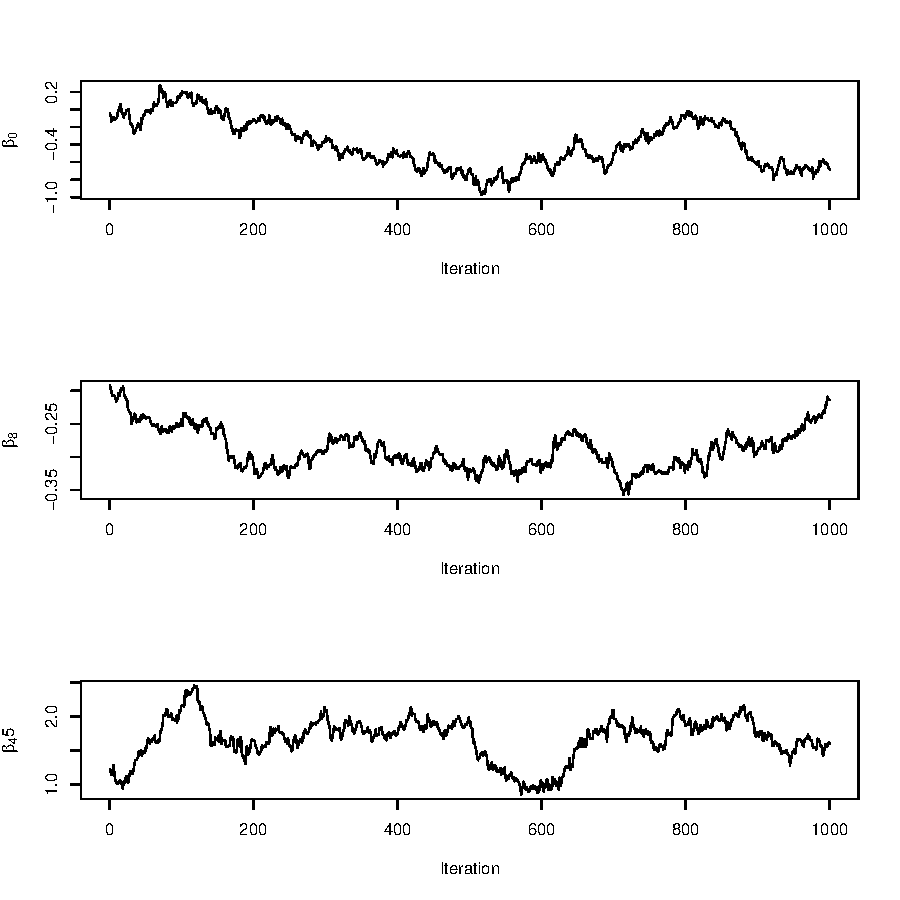
\includegraphics[width=1\textwidth]{traceplot_poisson_zip_da.pdf}
 \caption{Trace plots of three parameters from DA ZIP model}
 \end{subfigure}
  \hfill 
 \begin{subfigure}[b]{0.45\textwidth}
 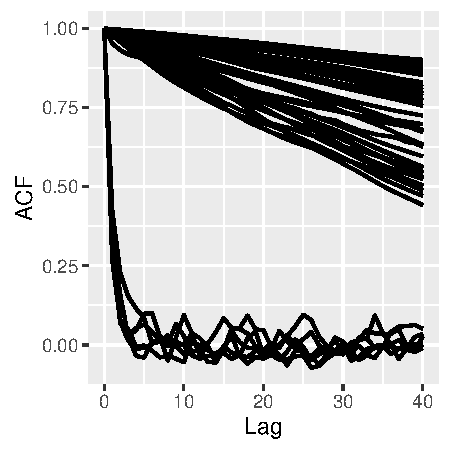
\includegraphics[width=1\textwidth]{poisson_zip_da_acf.pdf}
 \caption{Autocorrelation of all the 96 $\beta$'s from DA ZIP model.}
 \end{subfigure}  
 \caption{The hierarchy in the zero-inflated Poisson model does NOT help reduce the autocorrelation.}
 \end{figure}



\subsection{Goodness-of-Fit and Cross-Validation for Poisson Regression}


 \begin{figure}[H]
 % \centering
   \begin{subfigure}[b]{0.45\textwidth}
 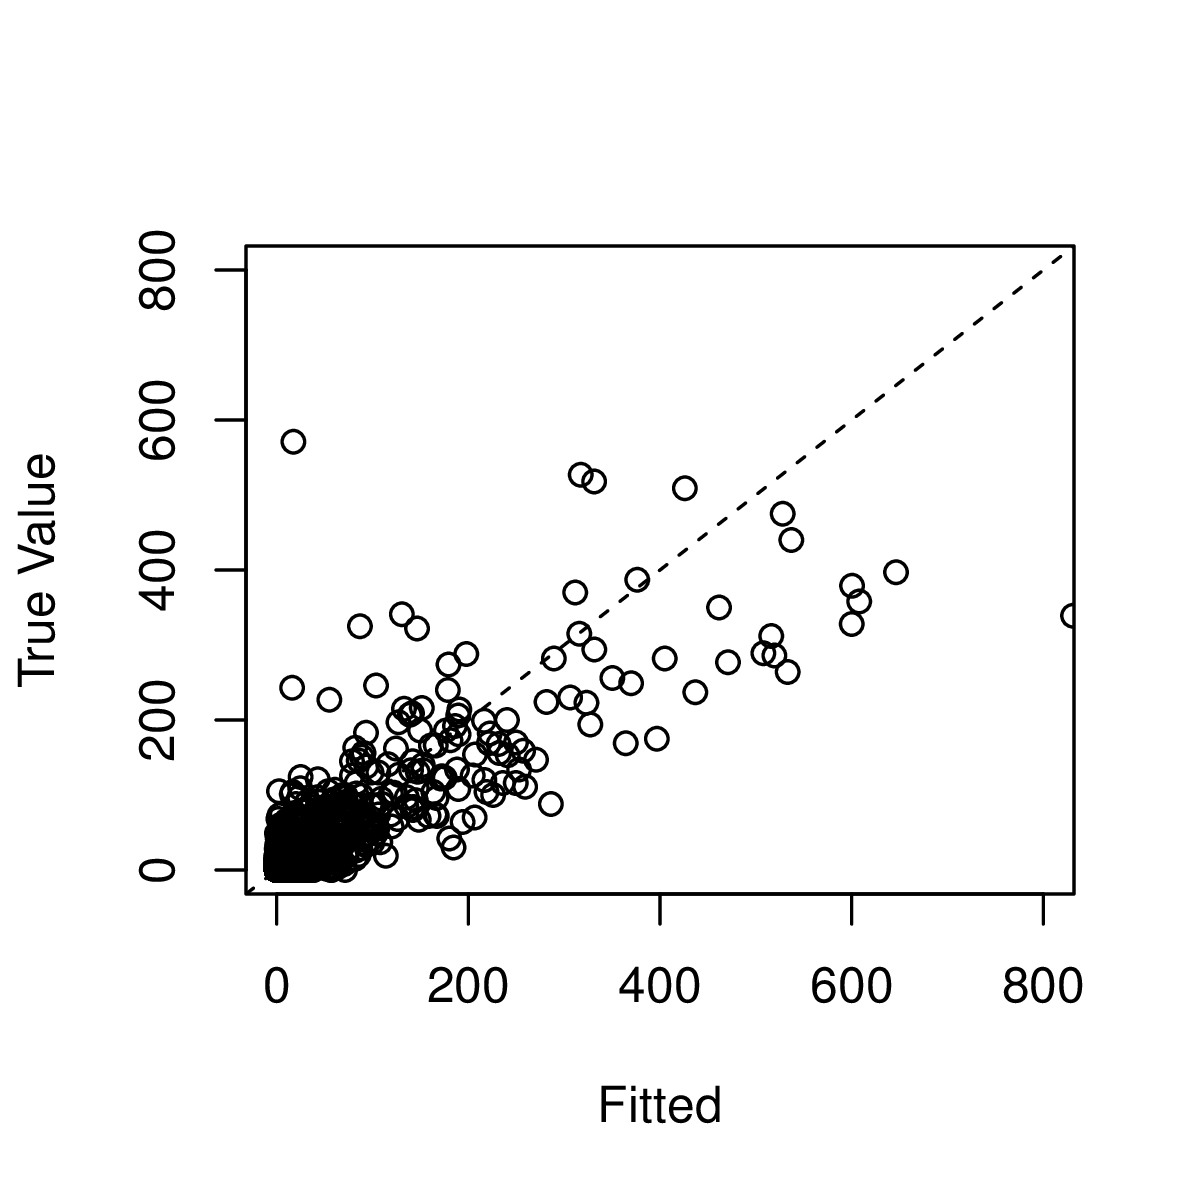
\includegraphics[width=1\textwidth]{poisson_fitting_da.png}
 \caption{Fitted vs true values using DA}
 \end{subfigure}
  \hfill 
 \begin{subfigure}[b]{0.45\textwidth}
 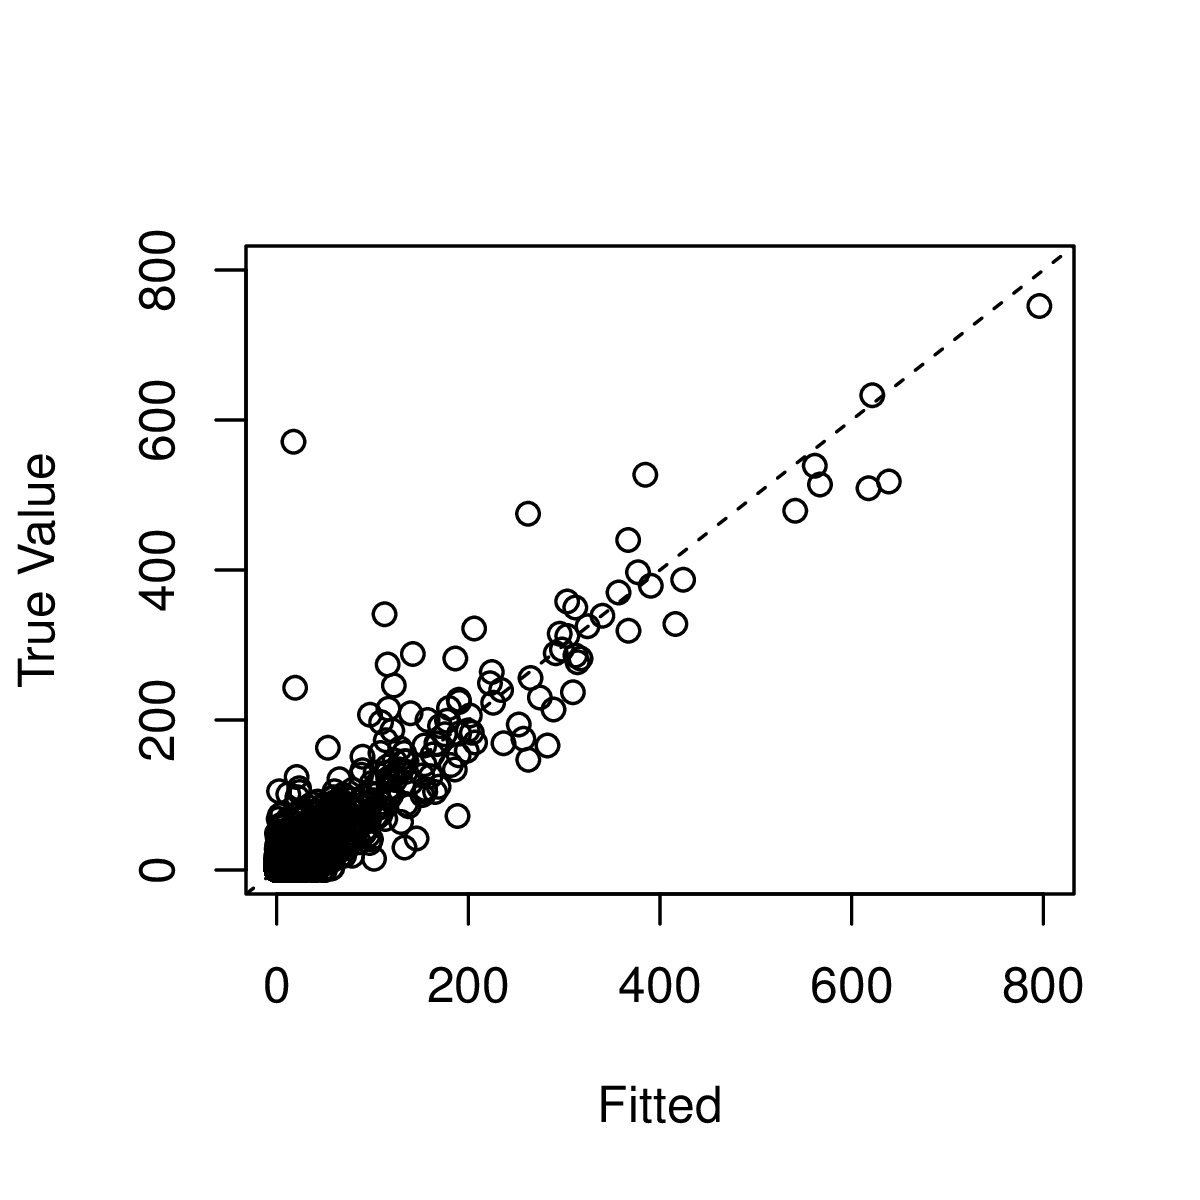
\includegraphics[width=1\textwidth]{poisson_fitting_ada.png}
 \caption{Fitted vs true values using CDA}
 \end{subfigure}  
   \begin{subfigure}[b]{0.45\textwidth}
 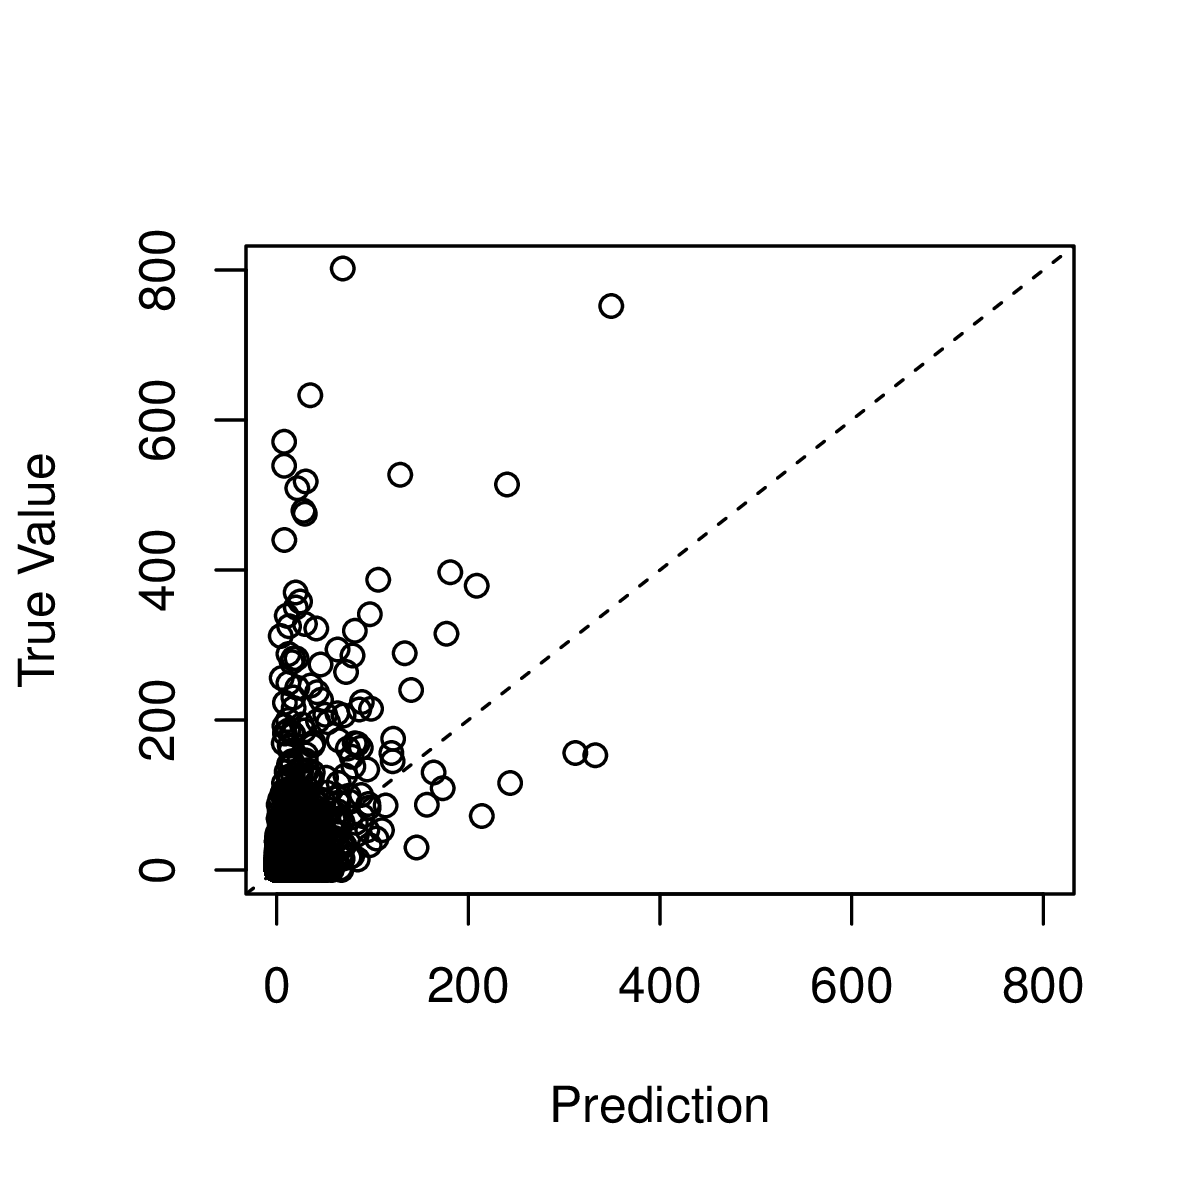
\includegraphics[width=1\textwidth]{poisson_cv_da.png}
 \caption{Prediction vs true values using DA}
 \end{subfigure}
  \hfill 
 \begin{subfigure}[b]{0.45\textwidth}
 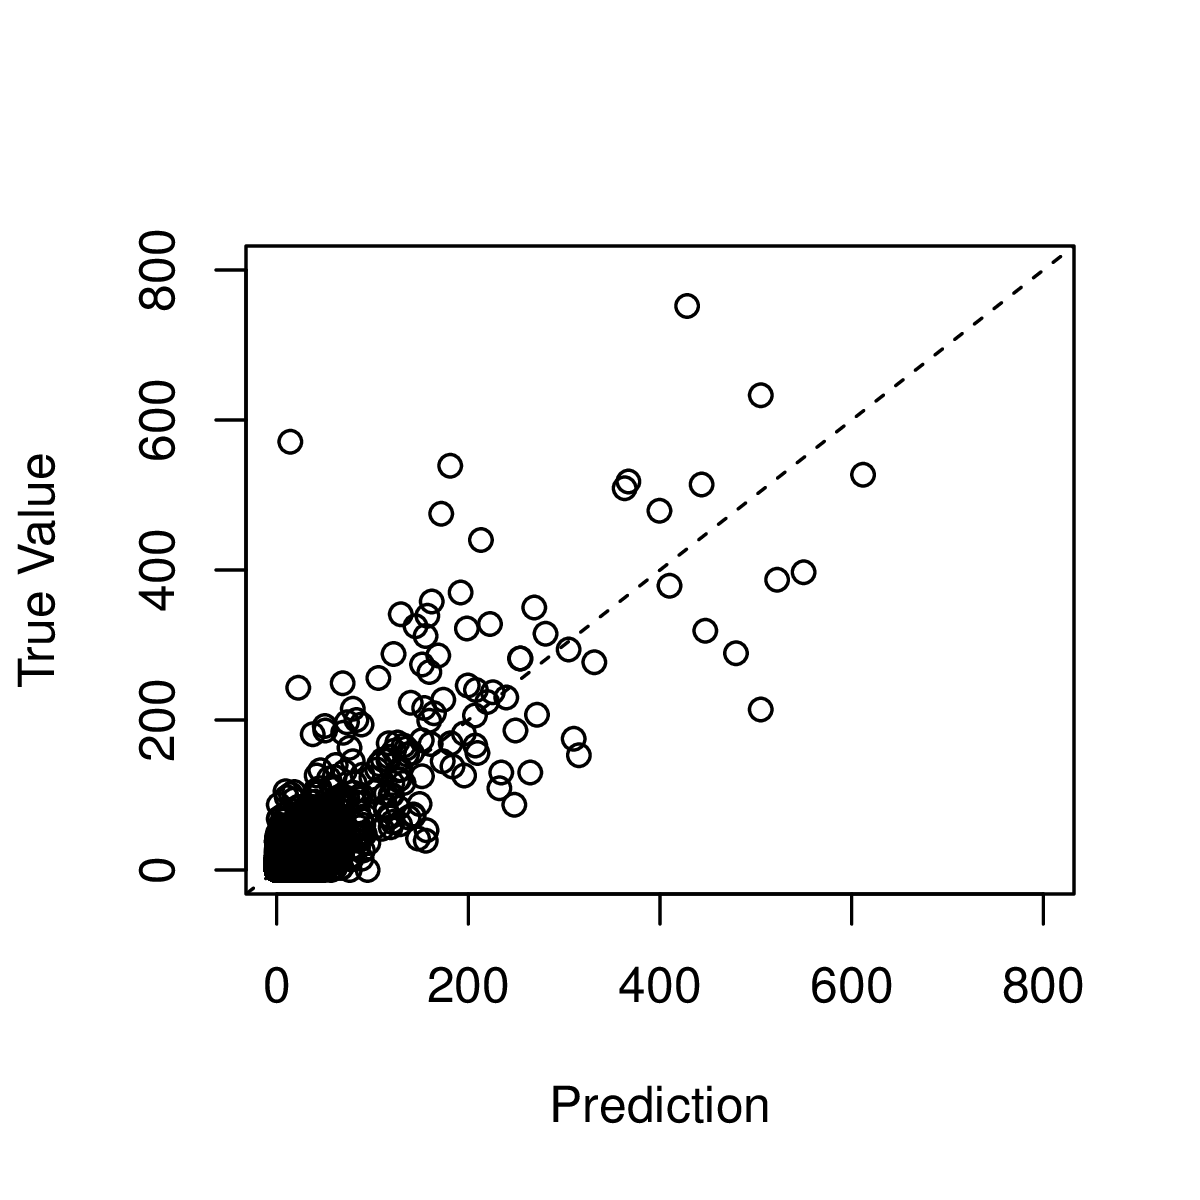
\includegraphics[width=1\textwidth]{poisson_cv_ada.png}
 \caption{Prediction vs true values using CDA}
 \end{subfigure} 
 \caption{The posterior estimates produced by CDA is better fitted to the data and have more accurate prediction than DA.}
 \end{figure}

 \subsection{Comparing posterior samples of CDA with HMC}


\begin{figure}[H]
 % \centering
   \begin{subfigure}[b]{0.45\textwidth}
 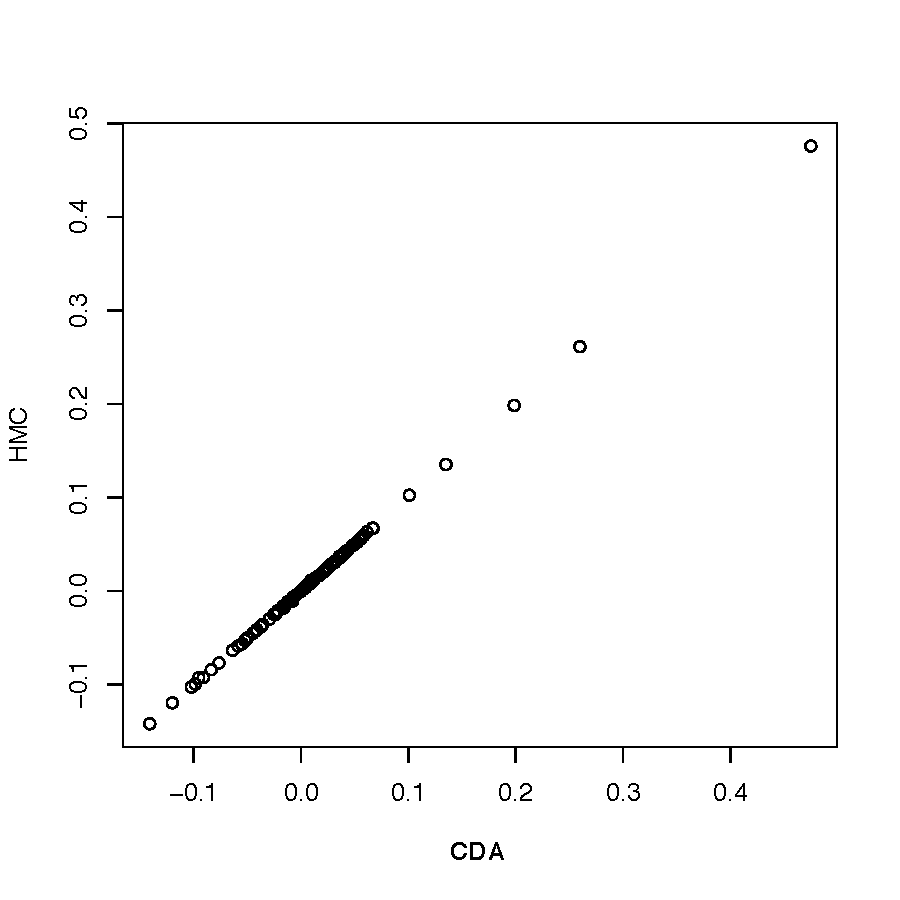
\includegraphics[width=1\textwidth]{CDAvsHMC_mean.pdf}
 \caption{Comparing posterior means for $\beta_1,\dots \beta_{95}$ from the HMC and CDA.}
 \end{subfigure}
  \hfill 
 \begin{subfigure}[b]{0.45\textwidth}
 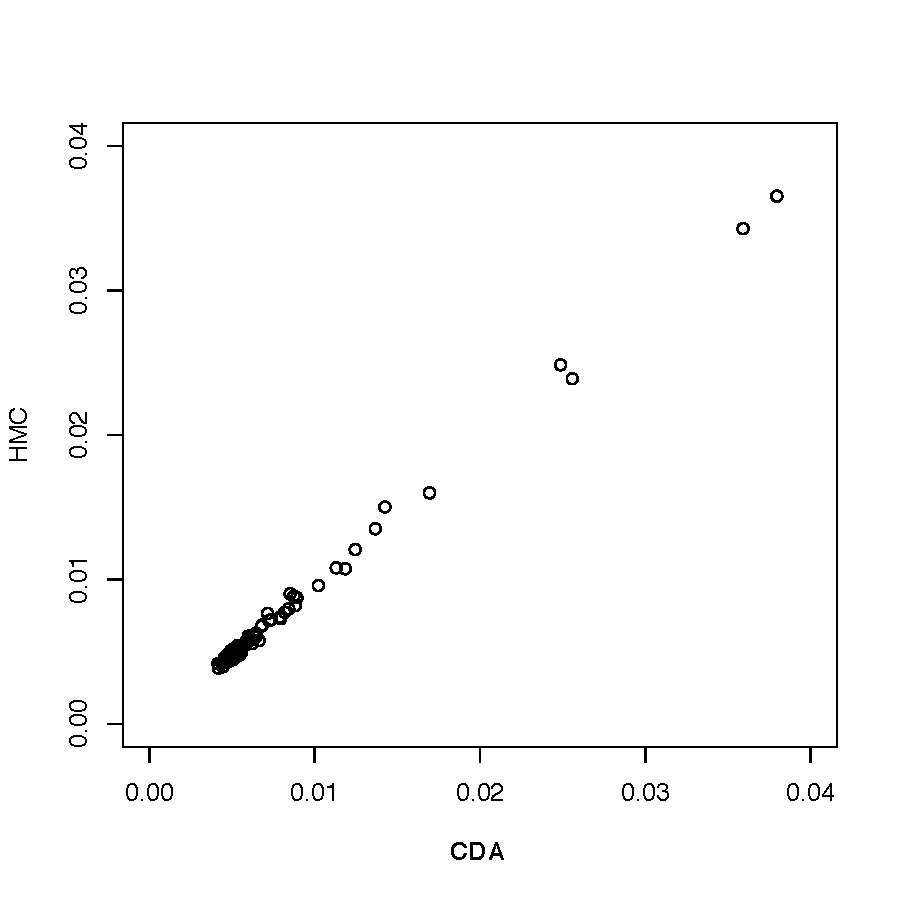
\includegraphics[width=1\textwidth]{CDAvsHMC_sd.pdf}
 \caption{Comparing posterior standard deviation for $\beta_1,\dots \beta_{95}$ from the HMC and CDA.}
 \end{subfigure}  
 \caption{The results from CDA and HMC agree very well.}
 \end{figure}

\subsection{Mixing of HMC}


 \begin{figure}[H]
 % \centering
   \begin{subfigure}[b]{0.45\textwidth}
 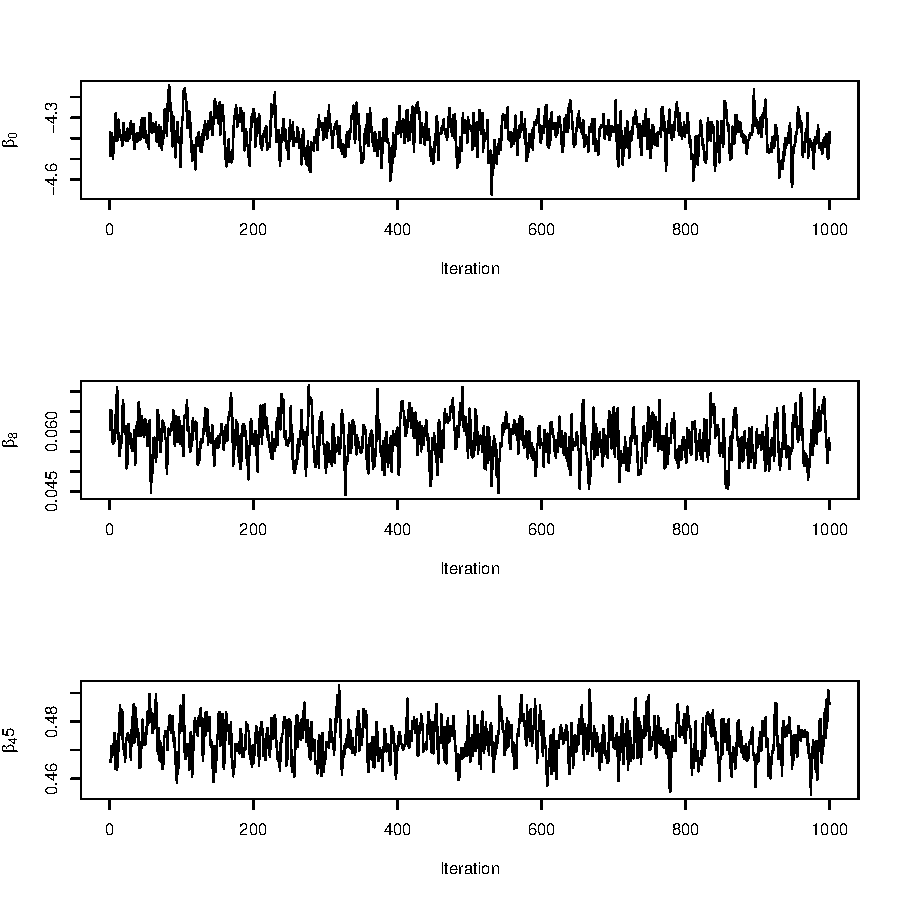
\includegraphics[width=1\textwidth]{traceplot_poisson_ada.pdf}
 \caption{Traceplots}
 \end{subfigure}
  \hfill 
 \begin{subfigure}[b]{0.45\textwidth}
 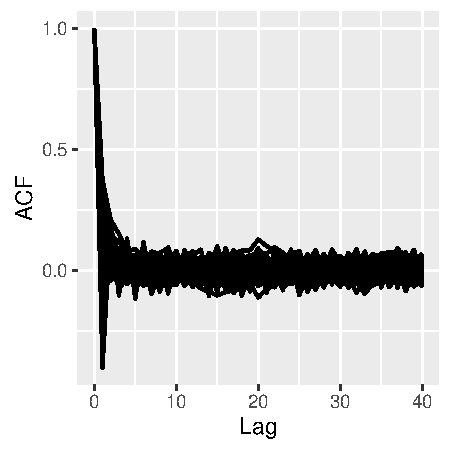
\includegraphics[width=1\textwidth]{poisson_hmc_acf.pdf}
 \caption{Autocorrelation}
 \end{subfigure}  
 \caption{The posterior estimates produced by HMC.}
 \end{figure}
 


 
\end{document}




